% SMS in CHC -- manuscript draft.
% Typography and notation: Gauge Boson Signal.tex.
% Front-matter structure: Qin and Xianyu (2023), Closed-Form Formulae
% for Inflation Correlators (local PDF in ref/).
% Sections 2.1--2.4 and the associated integral appendices are populated.
% Build: latexmk -pdf -interaction=nonstopmode -halt-on-error "SMS in CHC.tex"

\documentclass[a4paper,12pt]{article}
%\usepackage[lite,subscriptcorrection,slantedGreek,nofontinfo]{mtpro2}
%\usepackage{times} 
\usepackage{amsfonts}
\usepackage{mathrsfs}
\usepackage{amsmath}
\usepackage{amssymb}
\usepackage{framed}
%\usepackage{mathptmx}
\usepackage[medium]{titlesec}
\usepackage{bm}
\usepackage{cite}                                                   
%\usepackage{feynmp-auto}
\usepackage[normalem]{ulem}
\usepackage{extarrows}
\usepackage{slashed}
\usepackage{isodateo}
\usepackage{graphicx}
\usepackage{tikz}
\usepackage{placeins}
\usepackage{xcolor}
\usepackage[bookmarksnumbered=true,bookmarksopen=true]{hyperref}
 \hypersetup{colorlinks,%
             linkcolor=[rgb]{0,0.3,0.6}, %
             citecolor=[rgb]{0,0.3,0.6}, %
             urlcolor=[rgb]{0,0.3,0.6}}
\usepackage[hmargin=.7in,vmargin=1.1in]{geometry}
\usepackage{indentfirst}
\usepackage{booktabs}

\linespread{1.1}
%\numberwithin{equation}{section}
\newcommand{\FR}[2]{\displaystyle\frac{\,{#1}\,}{#2}}
\newcommand{\fr}[2]{\mbox{$\frac{\,{#1}\,}{#2}$}}
\newcommand{\n}{\nonumber}
\renewcommand{\rm}{\mathrm}
\renewcommand{\thefootnote}{\arabic{footnote}}

\newcommand{\red}{\color{red}}
\newcommand{\blue}{\color{blue}}
\newcommand{\gray}{\color{gray}}
\newcommand{\hl}{\color[rgb]{1,0,.5}}

\def\bge{\begin{equation}}
\def\ede{\end{equation}}
\def\bga{\begin{aligned}}
\def\eda{\end{aligned}}
\def\bgb{\begin{bmatrix}}
\def\edb{\end{bmatrix}}
\def\bgp{\begin{pmatrix}}
\def\edp{\end{pmatrix}}
\def\bgm{\begin{matrix}}
\def\edm{\end{matrix}}
\def\bgs{\begin{subequations}}
\def\eds{\end{subequations}}
\newcommand{\order}[1]{\mathcal{O}({#1})}
\def\di{{\mathrm{d}}}
\def\D{{\mathrm{D}}}
\def\Di{{\mathcal{D}}}

\def\T{\mathcal{T}}
\def\J{\mathcal{J}}
\def\mb{\mathbf}
\def\ms{\mathscr}
\def\mf{\mathfrak}
\def\mc{\mathcal}
\def\cl{\mathrm{cl}}
\def\pd{\partial}
\def\ld{{\mathscr{L}}}
\def\hd{{\mathscr{H}}}
\def\z{{\bar{z}}}
\def\la{\langle}\def\ra{\rangle}
\def\sla{\slashed}
\def\const{\mathrm{const.}}
\setlength\unitlength{1mm}
\def\tr{\mathrm{\,tr\,}}
\def\Tr{\mathrm{\,Tr\,}}
\def\Det{\mathrm{\,Det\,}}
\def\to{\rightarrow}
\def\To{\Rightarrow}
\def\ii{\mathrm{i}}

\def\al{\alpha}
\def\be{\beta}
\def\ga{\gamma}
\def\de{\delta}
\def\ep{\epsilon}
\def\ka{\kappa}
\def\lam{\lambda}
\def\rh{\rho}
\def\si{\sigma}
\def\ze{\zeta}
\def\tn{\tilde\nu}


\def\Wh{\mathrm{W}}


\def\aa{\mathsf{a}}
\def\bb{\mathsf{b}}
\def\cc{\mathsf{c}}
\def\dd{\mathsf{d}}

\def\C{\mathbb{C}}
\def\R{\mathbb{R}}

\def\Mp{M_{\text{Pl}}}


\def\Re{\mathrm{Re}\,}
\def\Im{\mathrm{Im}\,}

\def\ad{\mathrm{\,ad\,}}

\usepackage{mdframed} 
                   

\newmdenv[skipabove=0pt,%
          skipbelow=5pt,%
          leftmargin=0pt,%
          rightmargin=0pt,%
          innertopmargin=-5pt,%
          innerbottommargin=7pt,%
          innerleftmargin=2pt,%
          innerrightmargin=2pt,%
          splittopskip=0pt,%
          splitbottomskip=0pt,%
          linewidth=0pt,%
          nobreak=true]%
          {keyeqn2}                   
                   
                   
\newmdenv[backgroundcolor=gray!15,%
          skipabove=0pt,%
          skipbelow=5pt,%
          leftmargin=0pt,%
          rightmargin=0pt,%
          innertopmargin=-5pt,%
          innerbottommargin=7pt,%
          innerleftmargin=2pt,%
          innerrightmargin=2pt,%
          splittopskip=0pt,%
          splitbottomskip=0pt,%
          linewidth=0pt,%
          nobreak=true]%
          {keyeqn}

\usepackage{titlesec}          
\titleformat{\section}
{\normalfont\fontsize{15}{20}\bfseries}{\thesection}{1em}{}

\usepackage[T1]{fontenc}
\usepackage{lmodern}

\newcommand{\ob}[1]{\mkern 2mu \overline{\mkern -2mu #1 \mkern -2mu}\mkern 2mu}
\newcommand{\wt}[1]{\mkern 2mu \widetilde{\mkern -2mu #1 \mkern -2mu}\mkern 2mu}
\newcommand{\wh}[1]{\mkern 2mu \widehat{\mkern-2mu#1\mkern-2mu}\mkern 2mu}

\newcommand{\fnemail}[1]{\footnote{Email: \href{mailto:#1}{\nolinkurl{#1}}}}

% \hypersetup{pdftitle={SMS in CHC}}
\setcounter{tocdepth}{2}

\title{\Large\textbf{Higgs Induced Signal in Cosmology}\\[2mm]}
\author{}
\date{}

\newcommand{\one}{\mathbf1_2}
\newcommand{\epsmat}{\boldsymbol{\epsilon}}
\newcommand{\Dsc}[1]{D^{\mathrm{sc},#1}}

\begin{document}

\maketitle

\vspace{20mm}
\begin{abstract}
% Abstract intentionally left blank.
\vspace{10mm}
\end{abstract}

\clearpage
\tableofcontents

\clearpage
\section{Introduction}
\label{sec:introduction}
% Intentionally left blank.

\section{Gauge Boson Signal}
\label{sec:gauge-boson}
% Follow the calculation in Gauge Boson Signal.tex and its companion PDF.

\subsection{Preliminaries}
\label{sec:gauge-preliminaries}
We will compute the connected four-point function
$\langle\delta h_{\mb k_1}\delta h_{\mb k_2}
\delta h_{\mb k_3}\delta h_{\mb k_4}\rangle'$
generated by a massive gauge-boson loop. 
Our interest is the leading nonlocal signal in the collapsed $s$ channel,
\begin{equation}
    \mb k_s\equiv\mb k_1+\mb k_2=-(\mb k_3+\mb k_4),
    \qquad k_s\ll k_i,\qquad
    k_{12}\equiv k_1+k_2,\quad k_{34}\equiv k_3+k_4,
    \label{eq:collapsed-kinematics}
\end{equation}
where $k_i\equiv|\mb k_i|$. Thus $k_1\simeq k_2$ and
$k_3\simeq k_4$ at leading order. 
We choose $\mb k_s$ along the
$z$ axis and set the azimuth of $\mb k_1$ to zero. Here $\theta_1$ and
$\theta_3$ are the polar angles of $\mb k_1$ and $\mb k_3$, respectively, and
$\phi_3$ is their relative azimuth.

The Higgs--gauge couplings follow from the Higgs kinetic term
\cite{lu_cosmological_2020}:
\begin{equation}
    \frac{\sqrt{-g}}{2}|\mathrm D_\mu\mb H|^2
    \supset\frac{a^2g^2}{4}(h_0+\delta h)^2
    \left(W^+_\mu W^{-\mu}+\frac{Z_\mu Z^\mu}{2c_W^2}\right),
    \label{eq:higgs-gauge-couplings}
\end{equation}
where $g$ is the weak gauge coupling, $c_W=\cos\theta_W$, and the
Lorentz contractions on the right use the flat conformal metric.
The terms linear and quadratic in $\delta h$ generate the cubic and
quartic vertices, respectively. 
They give the bubble, two triangle placements, and box shown in
Fig.~\ref{fig:gauge-diagrams}.

\begin{figure}[htbp]
    \centering
    \begin{minipage}[c]{0.48\textwidth}
        \centering
        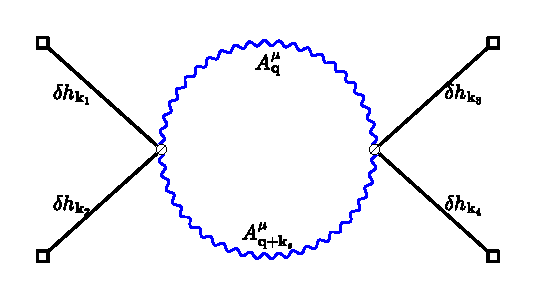
\includegraphics[height=3.2cm]{figure/Bub.pdf}
        \par\smallskip (a) Bubble
    \end{minipage}\hfill
    \begin{minipage}[c]{0.48\textwidth}
        \centering
        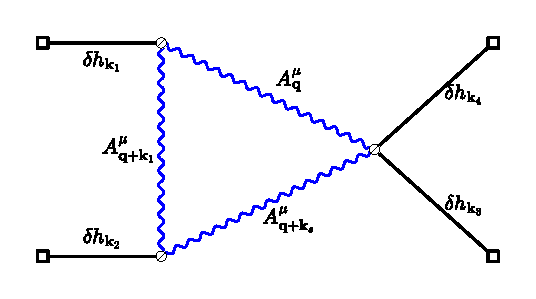
\includegraphics[height=3.2cm]{figure/Tri1.pdf}
        \par\smallskip (b) Triangle 1
    \end{minipage}
    \par\medskip
    \begin{minipage}[c]{0.48\textwidth}
        \centering
        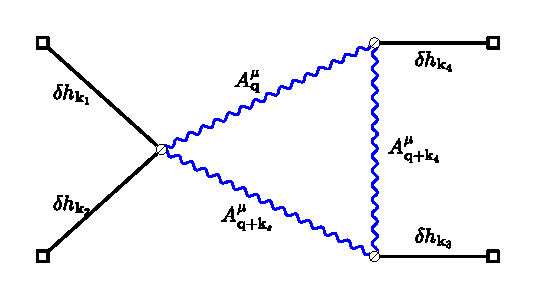
\includegraphics[height=3.2cm]{figure/Tri2.pdf}
        \par\smallskip (c) Triangle 2
    \end{minipage}\hfill
    \begin{minipage}[c]{0.48\textwidth}
        \centering
        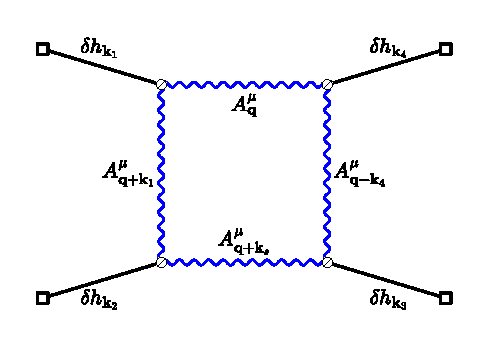
\includegraphics[height=3.2cm]{figure/Box.pdf}
        \par\smallskip (d) Box
    \end{minipage}
    \caption{The four gauge-boson loop diagrams considered here.
    Black solid lines denote external Higgs modes and blue wavy
    lines denote gauge-boson propagators. }
    \label{fig:gauge-diagrams}
\end{figure}

In the light-Higgs regime, the dominant
infrared Higgs-loop contribution to the vector masses is
\cite{lu_cosmological_2020}
\begin{equation}
    m_W^2\simeq\frac{3g^2H^4}{8\pi^2m_H^2},\qquad
    m_Z^2\simeq\frac{m_W^2}{c_W^2}.
    \label{eq:gauge-masses}
\end{equation}
Here $m_H$ is the effective Higgs mass. We use a constant vector mass
$m_V$ and the parameter
$\tilde\nu\equiv\sqrt{m_V^2/H^2-1/4}>0$ in the following.
The $W$ and $Z$ contributions are obtained with their respective masses
and couplings in \eqref{eq:higgs-gauge-couplings}.

We use $\lambda,\sigma=L,+,-,T$ for vector polarization-basis labels, and
$\eta=\pm1$ for the two nonlocal branches. 
Neglecting the Higgs mass
in the external mode functions, we write its bulk-to-boundary propagator as
\begin{equation}
    G_{\aa}(k;\tau)=\frac{H^2}{2k^3}
    (1-\ii\aa k\tau)e^{\ii\aa k\tau}.
    \label{eq:higgs-propagator}
\end{equation}
The spacetime vector propagator decomposes as
\begin{align}
    D_{\aa\bb,\mu\nu}(\mb k;\tau_1,\tau_2)
    ={}&\sum_{\lambda=T,L,\pm}
    e^{(\lambda)}_{\mb k,\mu}e^{(\lambda)*}_{\mb k,\nu}
    D^{(\lambda)}_{\aa\bb}(k;\tau_1,\tau_2)
    \nonumber\\
    &+e^{(T)}_{\mb k,\mu}e^{(L)*}_{\mb k,\nu}
    D^{(TL)}_{\aa\bb}(k;\tau_1,\tau_2)
    +e^{(L)}_{\mb k,\mu}e^{(T)*}_{\mb k,\nu}
    D^{(LT)}_{\aa\bb}(k;\tau_1,\tau_2),
    \label{eq:polarization-decomposition}
\end{align}
where $\mu,\nu=0,1,2,3$. In the comoving frame, the covariant
polarization basis is \cite{qin_helical_2023}
\[
    e^{(T)}_{\mb k,\mu}=(1,\mb0),\qquad
    e^{(L)}_{\mb k,\mu}=(0,\widehat{\mb k}),\qquad
    e^{(\pm)}_{\mb k,\mu}
    =\frac1{\sqrt2}(0,\mb e_\theta\pm\ii\mb e_\phi),
\]
with $(\widehat{\mb k},\mb e_\theta,\mb e_\phi)$ the orthonormal
spherical basis. 
The label $T$ denotes the temporal component of the longitudinal mode.

At zero chemical potential, all components can be expressed through an auxiliary scalar
propagator with the same Hankel index
\cite{qin_helical_2023,qin_closed-form_2023}:
\begin{align}
    D^{\rm(s)}_>(k;\tau_1,\tau_2)
    &=\frac{\pi H^2}{4}e^{-\pi\tilde\nu}
    (\tau_1\tau_2)^{3/2}
    \mathrm H^{(1)}_{\ii\tilde\nu}(-k\tau_1)
    \mathrm H^{(2)}_{-\ii\tilde\nu}(-k\tau_2),
    \label{eq:scalar-propagator}\\
    D^{(\pm)}_>&=\frac{D^{\rm(s)}_>}{H^2\tau_1\tau_2},\qquad
    D^{(L)}_>=\frac{(\partial_{\tau_1}-2/\tau_1)
    (\partial_{\tau_2}-2/\tau_2)D^{\rm(s)}_>}
    {H^2(\tilde\nu^2+1/4)},
    \label{eq:vector-scalar-relation}\\
    D^{(T)}_>&=\frac{k^2D^{\rm(s)}_>}
    {H^2(\tilde\nu^2+1/4)},
    \label{eq:temporal-scalar-relation}\\
    D^{(TL)}_>&=\frac{\ii k(\partial_{\tau_2}-2/\tau_2)D^{\rm(s)}_>}
    {H^2(\tilde\nu^2+1/4)},\qquad
    D^{(LT)}_>=-\frac{\ii k(\partial_{\tau_1}-2/\tau_1)D^{\rm(s)}_>}
    {H^2(\tilde\nu^2+1/4)}.
    \label{eq:mixed-scalar-relations}
\end{align}

With spacetime indices and momentum arguments suppressed,
$D_{-+}=D_>$, $D_{+-}=D_<$, and the separated-time SK propagators are
\begin{align}
    D_{++}&=\theta(\tau_1-\tau_2)D_>
              +\theta(\tau_2-\tau_1)D_<,\nonumber\\
    D_{--}&=\theta(\tau_2-\tau_1)D_>
              +\theta(\tau_1-\tau_2)D_<.
    \label{eq:sk-prescription}
\end{align}
These relations apply to $D^{(\pm)},D^{(L)},D^{(TL)}$ and $D^{(LT)}$. 
But for $D^{(T)}$, the $++$ and $--$ propagators have a delta-function term because the temporal mode is not a physical degree of freedom:
\begin{align}
    D_{++}^{(T)}&=\theta(\tau_1-\tau_2)D_>^{(T)}
              +\theta(\tau_2-\tau_1)D_<^{(T)} + \frac{\ii \delta(\tau_1-\tau_2)}{H^2(\tn^2+1/4) a(\tau_1)^2} ,\nonumber\\
    D_{--}^{(T)}&=\theta(\tau_2-\tau_1)D_>^{(T)}
              +\theta(\tau_1-\tau_2)D_<^{(T)} - \frac{\ii \delta(\tau_1-\tau_2)}{H^2(\tn^2+1/4) a(\tau_1)^2} .
\end{align}
Then we will see that the propagators $D^{(T)},D^{(TL)}$ and $D^{(LT)}$ will not contribute to the leading nonlocal signal.

The leading nonlocal parts of the spatial propagators are independent
of the SK indices:
\begin{align}
    \left[D^{(\pm)}_{\aa\bb}(k;\tau_1,\tau_2)\right]_{\rm NonL}
    &=\frac{(\tau_1\tau_2)^{1/2}}{4\pi}
      \sum_{\eta=\pm1}\Gamma^2(-\ii\eta\tilde\nu)
      \left(\frac{k^2\tau_1\tau_2}{4}\right)^{\ii\eta\tilde\nu},
      \label{eq:transverse-nonlocal}\\
    \left[D^{(L)}_{\aa\bb}(k;\tau_1,\tau_2)\right]_{\rm NonL}
    &=\frac{(\tau_1\tau_2)^{1/2}}{4\pi}
      \sum_{\eta=\pm1}
      \frac{(-1/2+\ii\eta\tilde\nu)^2}{\tilde\nu^2+1/4}
      \Gamma^2(-\ii\eta\tilde\nu)
      \left(\frac{k^2\tau_1\tau_2}{4}\right)^{\ii\eta\tilde\nu}.
    \label{eq:longitudinal-nonlocal}
\end{align}
The temporal nonlocal part is
\begin{equation}
    \left[D^{(T)}_{\aa\bb}(k;\tau_1,\tau_2)\right]_{\rm NonL}
    =\frac{k^2(\tau_1\tau_2)^{3/2}}
    {4\pi(\tilde\nu^2+1/4)}
    \sum_{\eta=\pm1}\Gamma^2(-\ii\eta\tilde\nu)
    \left(\frac{k^2\tau_1\tau_2}{4}\right)^{\ii\eta\tilde\nu}.
    \label{eq:temporal-nonlocal}
\end{equation}

The one-loop factorization theorem and cutting rule
\cite{qin_inflation_2023} isolate the leading nonlocal signal in the
collapsed channel. We first identify the two internal lines whose
removal separates the external pairs $(1,2)$ and $(3,4)$.
Their momenta can be chosen as $\mb q$ and
$\mb K\equiv\mb q+\mb k_s$. The relevant loop region has
$q,K\sim k_s\ll k_i$. We replace these two propagators by the
leading nonlocal terms of their late-time expansions, keeping their
polarization tensors, and expand the remaining hard propagators
to leading order in the soft momenta. The hard propagators retain
their full time dependence and SK ordering.

The cut propagators are independent of the SK indices, and their
time dependence separates between the two endpoints. The time
integrals thus factorize into two tree subgraphs with additional
time powers supplied by the cut lines. Multiplying these subgraphs
by the soft momentum integral and summing over polarizations gives
the nonlocal signal. 
The branches $\eta=\pm1$ combine into the oscillatory signal
retained below. Higher terms in the soft expansion give subleading
corrections in the collapsed limit.

The propagators $D^{(T)}$, $D^{(TL)}$, and $D^{(LT)}$ do not
contribute to the leading nonlocal signal. On a soft line, each
temporal mode function $B^{(T)}$ carries an additional factor of
$k\tau$ relative to the spatial modes $B^{(L)}$ and $B^{(\pm)}$.
Their nonanalytic contributions are therefore suppressed in the
collapsed limit. The contact term in $D^{(T)}$ is analytic in the
soft momentum and does not contribute to the nonlocal signal.
On a hard line, a temporal endpoint has a vanishing polarization
contraction with the spatial components of the attached soft line.
A nonzero contraction would require a temporal soft component,
which is already suppressed. We therefore omit propagators with
temporal components when computing the leading signal below.

All required soft momentum integrals reduce to five dimensionless
functions $f_r$, $r=0,1,2,3,4$. With
$z\equiv\widehat{\mb q}\cdot\widehat{\mb k}_s$, we define
\begin{equation}
    \int\frac{\di^3\mb q}{(2\pi)^3}
    q^{-2\alpha}K^{-2\beta}z^r
    =\frac{k_s^{3-2\alpha-2\beta}}{(4\pi)^{3/2}}
    f_r(\alpha,\beta),\qquad r=0,1,2,3,4.
    \label{eq:fr-definition}
\end{equation}
These expressions are understood by analytic continuation from the
convergent domain. The first three functions are
\begin{align}
    f_0(\alpha,\beta)
    &=\frac{\Gamma(\alpha+\beta-3/2)
    \Gamma(3/2-\alpha)\Gamma(3/2-\beta)}
    {\Gamma(3-\alpha-\beta)\Gamma(\alpha)\Gamma(\beta)},
    \label{eq:f0}\\
    f_1(\alpha,\beta)
    &=\frac12\left[
    f_0(\alpha+\tfrac12,\beta-1)
    -f_0(\alpha-\tfrac12,\beta)
    -f_0(\alpha+\tfrac12,\beta)\right],
    \label{eq:f1}\\
    f_2(\alpha,\beta)
    &=\frac14\left[
    f_0(\alpha+1,\beta-2)+f_0(\alpha-1,\beta)
    +f_0(\alpha+1,\beta)\right.\nonumber\\
    &\hspace{13mm}\left.
    -2f_0(\alpha,\beta-1)-2f_0(\alpha+1,\beta-1)
    +2f_0(\alpha,\beta)\right].
    \label{eq:f2}
\end{align}
The functions $f_3$ and $f_4$ are likewise finite sums of $f_0$;
their explicit expressions are collected in App.~\ref{app:loop-integrals}.

For the nonlocal branch $\eta$, it is convenient to set
$x=-\ii\eta\tilde\nu$ and define
\begin{equation}
    \mathcal J_r(m,n;x)
    \equiv f_r\left(x-\frac m2,x+\frac n2\right),
    \qquad r=0,1,2,3,4.
    \label{eq:Jr-definition}
\end{equation}
Here $m,n$ are integer shifts of momentum powers, unrelated to $m_V$.
In particular,
\begin{equation}
    \int\frac{\di^3\mb q}{(2\pi)^3}
    \left(\frac q2\right)^{-2x}
    \left(\frac K2\right)^{-2x}q^mK^{-n}z^r
    =\frac{4^{2x}k_s^{3-4x+m-n}}{(4\pi)^{3/2}}
    \mathcal J_r(m,n;x).
    \label{eq:Jr-normalization}
\end{equation}

\FloatBarrier
\subsection{Bubble Diagram}
\label{sec:gauge-bubble}
The bubble contains two quartic vertices, each attached to a pair of external Higgs modes. 
With the four external momenta understood, the $s$-channel contribution is
\begin{align}
    \langle\delta h^4\rangle'_{\mathrm{Bub}}
    ={}&\frac{g^4}{8}
    \sum_{\aa,\bb=\pm1}(-\aa\bb)
    \int_{-\infty}^{0}\frac{\di\tau_1}{|H\tau_1|^2}
    \int_{-\infty}^{0}\frac{\di\tau_2}{|H\tau_2|^2}
    G_{\aa}(k_1;\tau_1)G_{\aa}(k_2;\tau_1)
    G_{\bb}(k_3;\tau_2)G_{\bb}(k_4;\tau_2)\nonumber\\
    &\times\int\frac{\di^3\mb q}{(2\pi)^3}
    D_{\aa\bb,ij}(\mb q;\tau_1,\tau_2)
    D_{\bb\aa,ji}(\mb K;\tau_2,\tau_1),
    \qquad \mb K=\mb q+\mb k_s.
    \label{eq:bubble-sk}
\end{align}
The symmetry factor $1/2$ is included. Throughout this section,
the $W^\pm$ contribution is obtained by multiplying the expressions
by $2$, and the $Z$ contribution by making the replacement $g\to g/c_W$,
with the corresponding mass used in each case.

Replacing the two soft propagators by
\eqref{eq:transverse-nonlocal}--\eqref{eq:longitudinal-nonlocal}
removes their SK-index dependence, as illustrated in
Fig.~\ref{fig:bubble-cutting}. After summing the polarizations,
the oscillatory part of the loop integral is
\begin{align}
    &\left[\int\frac{\di^3\mb q}{(2\pi)^3}
    D_{\aa\bb,ij}(\mb q;\tau_1,\tau_2)
    D_{\bb\aa,ji}(\mb K;\tau_2,\tau_1)\right]_{\rm NonL}
    \nonumber\\
    &\qquad\simeq\sum_{\eta=\pm1}
    (\tau_1\tau_2)^{1+2\ii\eta\tilde\nu}
    \frac{\Gamma^4(-\ii\eta\tilde\nu)}{(4\pi)^{7/2}}
    4^{-2\ii\eta\tilde\nu}k_s^{3+4\ii\eta\tilde\nu}
    \mathcal I_{g,\rm Bub}(-\ii\eta\tilde\nu).
    \label{eq:bubble-cut-loop}
\end{align}
\begin{figure}[htbp]
    \centering
    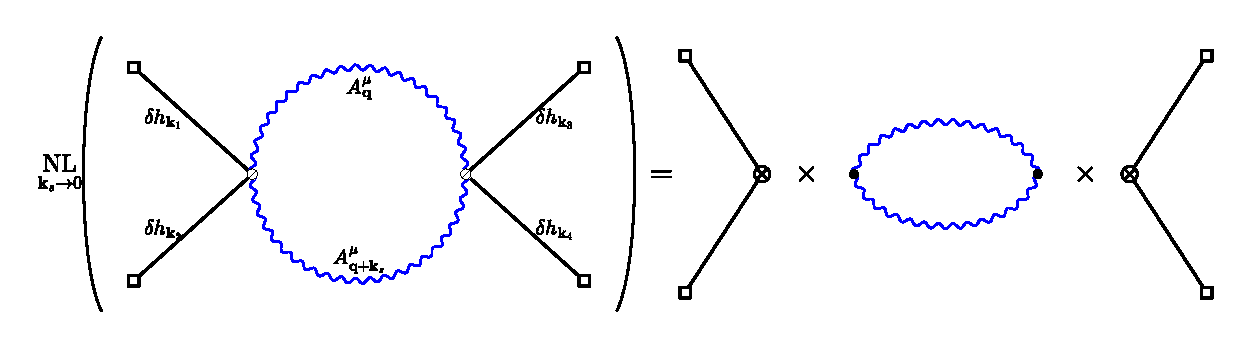
\includegraphics[width=\textwidth]{figure/Bub NL.pdf}
    \caption{The leading nonlocal part of the bubble in the
    $k_s\to0$ limit. The two soft gauge-boson lines supply the
    central loop factor, while the left and right subgraphs give
    the two quartic-vertex time integrals. Crossed circles mark
    the endpoints of the cut lines in the tree subgraphs.}
    \label{fig:bubble-cutting}
\end{figure}

The dimensionless polarization sum has the compact form
\begin{align}
    \mathcal I_{g,\rm Bub}(x)
    ={}&\frac{3+2x}{1-2x}\,\mathcal J_0(0,0;x)
    +\frac{16x^2}{(1-2x)^2}
    \left[\mathcal J_0(2,2;x)+2\mathcal J_1(1,2;x)
    +\mathcal J_2(0,2;x)\right],
    \label{eq:bubble-polarization-sum}
\end{align}
with $x=-\ii\eta\tilde\nu$ as in \eqref{eq:Jr-definition}.
The separate polarization contributions are given in
App.~\ref{app:bubble-polarizations}. 

The remaining time integrals factorize. For the left subgraph, at
$k_1\simeq k_2\simeq k_{12}/2$, we find
\begin{align}
    &\sum_{\aa=\pm1}\ii\aa
    \int_{-\infty}^{0}\frac{\di\tau}{|H\tau|^2}
    G_{\aa}(k_1;\tau)G_{\aa}(k_2;\tau)
    (-\tau)^{1+2\ii\eta\tilde\nu}
    \simeq\frac{H^2k_{12}^{-2\ii\eta\tilde\nu}}
    {4k_1^3k_2^3}\,\mathcal P^{(1)}_{g,\eta}(\tilde\nu),
    \label{eq:bubble-time-integral}\\
    &\mathcal P^{(1)}_{g,\eta}(\tilde\nu)
    =\frac{2+\ii\eta\tilde\nu}{2\ii\eta\tilde\nu}
    \ii\sinh(\pi\eta\tilde\nu)\Gamma(2+2\ii\eta\tilde\nu).
    \label{eq:bubble-P1}
\end{align}
The right vertex gives the same expression with
$(k_1,k_2,k_{12})\to(k_3,k_4,k_{34})$.
Combining the two vertices with \eqref{eq:bubble-cut-loop}, we obtain
\begin{equation}
    \left[\langle\delta h^4\rangle'_{\mathrm{Bub}}\right]_{\rm NonL}
    \simeq\frac{g^4H^4k_s^3}
    {128k_1^3k_2^3k_3^3k_4^3}
    \left[
    \left(\frac{k_s^2}{4k_{12}k_{34}}\right)^{2\ii\tilde\nu}
    C_g^{\rm Bub}(\tilde\nu)+\text{c.c.}\right],
    \label{eq:bubble-signal}
\end{equation}
where the complex signal coefficient is
\begin{equation}
    C_g^{\rm Bub}(\tilde\nu)
    =\frac{\Gamma^4(-\ii\tilde\nu)}{(4\pi)^{7/2}}
    \left[\mathcal P^{(1)}_{g,+}(\tilde\nu)\right]^2
    \mathcal I_{g,\rm Bub}(-\ii\tilde\nu).
    \label{eq:bubble-coefficient}
\end{equation}
This definition separates the loop and time integrals from the
couplings and diagram symmetry factor.
The bracket in \eqref{eq:bubble-signal} equals
\begin{equation}
    2|C_g^{\rm Bub}(\tilde\nu)|
    \cos\left[
    2\tilde\nu\log\!\left(\frac{k_s^2}{4k_{12}k_{34}}\right)
    +\arg C_g^{\rm Bub}(\tilde\nu)\right].
    \label{eq:bubble-phase}
\end{equation}

% Thus $|C_g^{\rm Bub}|$ and $\arg C_g^{\rm Bub}$ determine the amplitude
% and phase, respectively. Figure~\ref{fig:bubble-coefficient} shows their
% mass dependence, including the Boltzmann suppression of the amplitude.
% The $W$ and $Z$ signals are added using their respective
% $\tilde\nu_W$ and $\tilde\nu_Z$ in \eqref{eq:bubble-signal},
% with the multiplicity and coupling replacements stated above.
% The other exchange channels follow by permuting the external labels;
% \eqref{eq:bubble-signal} describes the leading signal in the
% $s$-channel collapsed limit.

\begin{figure}[tp]
    \centering
    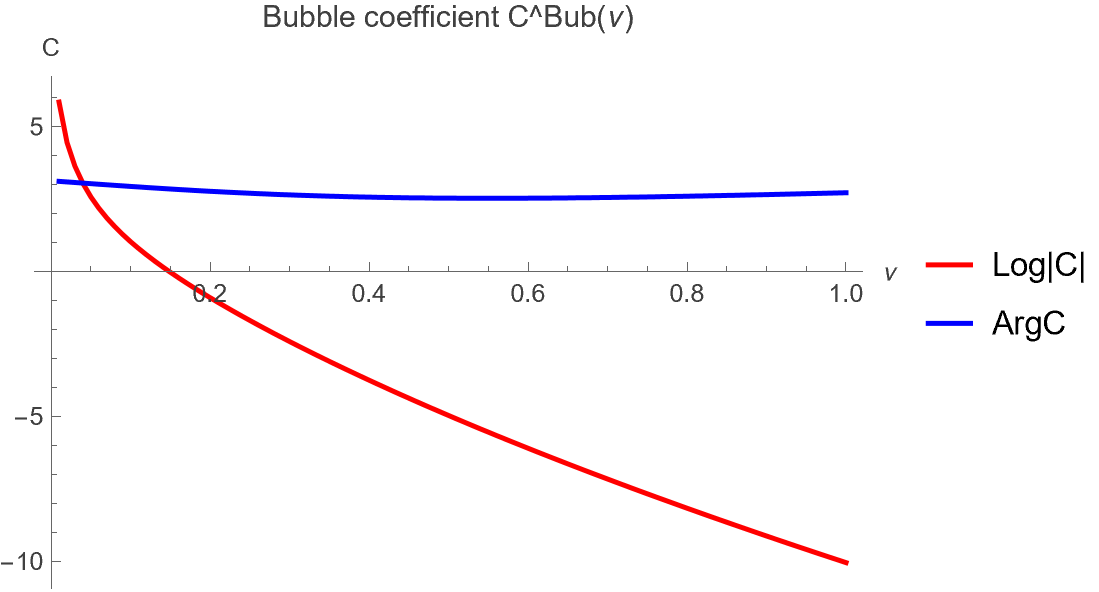
\includegraphics[width=0.80\textwidth]{figure/CBub.png}
    \caption{The bubble coefficient defined in \eqref{eq:bubble-coefficient}.
    The red and blue curves show $\log|C_g^{\rm Bub}|$ and
    $\arg C_g^{\rm Bub}$ in radians, respectively, as functions of
    $\tilde\nu$. }
    \label{fig:bubble-coefficient}
\end{figure}

% \clearpage

\FloatBarrier
\subsection{Triangle Diagram}
\label{sec:gauge-triangle}
The triangle contains two cubic vertices and one quartic vertex.
We first consider the diagram ``Triangle 1''.
The triangle has a unit diagram symmetry factor. 
In the conventions of Sec.~\ref{sec:gauge-bubble}, its integral expression is
\begin{align}
    \langle\delta h^4\rangle'_{\mathrm{Tri1}}
    ={}&\frac{g^6h_0^2}{8}
    \sum_{\aa,\bb,\cc=\pm1}(-\ii\aa\bb\cc)
    \int_{-\infty}^0\prod_{v=1}^{3}
    \frac{\di\tau_v}{|H\tau_v|^2}\,
    G_{\aa}(k_1;\tau_1)G_{\bb}(k_2;\tau_2)
    G_{\cc}(k_3;\tau_3)G_{\cc}(k_4;\tau_3)
    \nonumber\\
    &\times\int\frac{\di^3\mb q}{(2\pi)^3}
    D_{\aa\bb,ij}(\mb q+\mb k_1;\tau_1,\tau_2)
    D_{\bb\cc,j\ell}(\mb K;\tau_2,\tau_3)
    D_{\cc\aa,\ell i}(\mb q;\tau_3,\tau_1).
    \label{eq:triangle-sk}
\end{align}
The nonlocal signal comes from $q,K\sim k_s\ll k_1$.
We cut the $\mb q$ and $\mb K$ lines and evaluate the remaining hard
propagator at $\mb q+\mb k_1\simeq\mb k_1$. The latter retains its
full time dependence and SK ordering. The resulting factorization
is shown in Fig.~\ref{fig:triangle-cutting}.

\begin{figure}[htbp]
    \centering
    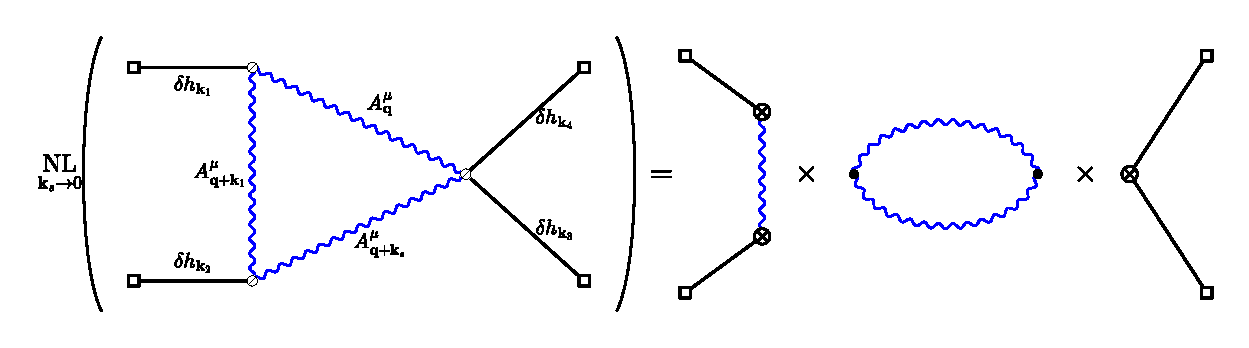
\includegraphics[width=\textwidth]{figure/Tri NL.pdf}
    \caption{The leading nonlocal part of the first triangle.
    Cutting the two soft lines leaves a hard gauge-boson exchange
    on the left and a quartic vertex on the right, joined by the
    central soft loop factor. The second triangle follows by
    exchanging the two external pairs.}
    \label{fig:triangle-cutting}
\end{figure}

After summing the soft polarizations, the cut loop takes the form
\begin{align}
    &\left[\int\frac{\di^3\mb q}{(2\pi)^3}
    D_{\aa\bb,ij}(\mb q+\mb k_1;\tau_1,\tau_2)
    D_{\bb\cc,j\ell}(\mb K;\tau_2,\tau_3)
    D_{\cc\aa,\ell i}(\mb q;\tau_3,\tau_1)\right]_{\rm NonL}
    \nonumber\\
    &\quad\simeq\sum_{\lambda=L,\pm}\sum_{\eta=\pm1}
    D^{(\lambda)}_{\aa\bb}(k_1;\tau_1,\tau_2)
    (\tau_1\tau_2)^{1/2+\ii\eta\tilde\nu}
    (-\tau_3)^{1+2\ii\eta\tilde\nu}
    \frac{\Gamma^4(-\ii\eta\tilde\nu)}{(4\pi)^{7/2}}
    4^{-2\ii\eta\tilde\nu}k_s^{3+4\ii\eta\tilde\nu}
    \mathcal I^\lambda_{g,\rm Tri}(-\ii\eta\tilde\nu,\theta_1).
    \label{eq:triangle-cut-loop}
\end{align}
This equation defines the dimensionless coefficients
$\mathcal I^\lambda_{g,\rm Tri}(x,\theta)$, with
$x=-\ii\eta\tilde\nu$. 
% Rotational symmetry and polarization
% completeness imply
% \begin{align}
%     \mathcal I^L_{g,\rm Tri}(x,\theta)
%     &=\sin^2\theta\,\mathcal I^L_{g,\rm Tri}(x,\pi/2)
%       +\cos^2\theta\,\mathcal I^L_{g,\rm Tri}(x,0),
%       \label{eq:triangle-angular-structure}\\
%     \mathcal I^+_{g,\rm Tri}(x,\theta)
%     &=\mathcal I^-_{g,\rm Tri}(x,\theta)
%       =\frac12\left[\mathcal I_{g,\rm Bub}(x)
%       -\mathcal I^L_{g,\rm Tri}(x,\theta)\right].
%       \label{eq:triangle-completeness}
% \end{align}
% Thus only one longitudinal coefficient is needed in addition to the bubble sum. 
% Its expression in terms of $\mathcal J_r$ is given in App.~\ref{app:triangle-coefficients}. 
After simplification, we surprisingly find that all three
coefficients equal $\mathcal I_{g,\rm Bub}(x)/3$ and the apparent angular
dependence cancels, as shown in \eqref{eq:triangle-I-closed}.

We next evaluate the left and right subgraphs.
The quartic vertex gives the time integral
$\mathcal P^{(1)}_{g,\eta}$ in \eqref{eq:bubble-P1}.
The two cubic vertices and the hard line instead define
\begin{align}
    &\sum_{\aa,\bb=\pm1}(-\aa\bb)
    \int_{-\infty}^0\frac{\di\tau_1\di\tau_2}
    {|H\tau_1|^2|H\tau_2|^2}
    G_{\aa}(k_1;\tau_1)G_{\bb}(k_2;\tau_2)
    D^{(\lambda)}_{\aa\bb}(k_1;\tau_1,\tau_2)
    (\tau_1\tau_2)^{1/2+\ii\eta\tilde\nu}
    \nonumber\\
    &\qquad\simeq
    \frac{k_{12}^{-2\ii\eta\tilde\nu}}{4k_1^3k_2^3}
    \mathcal P^{(2),\lambda}_{g,\eta}(\tilde\nu).
    \label{eq:triangle-time-integral}
\end{align}
At leading order, $k_1\simeq k_2\simeq k_{12}/2$.
The integral therefore reduces to the
double-folded scalar seeds of Ref.~\cite{qin_closed-form_2023},
which we denote by
$\mathcal M_{\aa\bb}^{p_1p_2}\equiv
\widetilde{\mathcal I}_{\aa\bb}^{p_1p_2}(1,1)$.
For the transverse modes this follows directly from
\eqref{eq:vector-scalar-relation}.
For the longitudinal mode, the differential relation also produces
a contact contribution \cite{qin_helical_2023}.
We retain this term together with the scalar-seed contributions.
The required seed exponents include
$p_0=-5/2+\ii\eta\tilde\nu$, on the boundary of the convergence
domain. We define the result by analytic continuation from
$p_0+\epsilon$, $\epsilon>0$, and take the finite part of the assembled
expression at $\epsilon=0$. The seed normalization, closed forms,
and combinations giving $\mathcal P^{(2),\lambda}_{g,\eta}$ are collected
in App.~\ref{app:triangle-coefficients}.

Finally, the leading signal of the first triangle is
\begin{equation}
    \left[\langle\delta h^4\rangle'_{\mathrm{Tri1}}\right]_{\rm NonL}
    \simeq\frac{g^6h_0^2H^2k_s^3}
    {128k_1^3k_2^3k_3^3k_4^3}
    \left[
    \left(\frac{k_s^2}{4k_{12}k_{34}}\right)^{2\ii\tilde\nu}
    C_g^{\rm Tri}(\tilde\nu)+\text{c.c.}\right],
    \label{eq:triangle-single-signal}
\end{equation}
where
\begin{equation}
    C_g^{\rm Tri}(\tilde\nu)
    =\frac{\Gamma^4(-\ii\tilde\nu)}{(4\pi)^{7/2}}
    \mathcal P^{(1)}_{g,+}(\tilde\nu)
    \sum_{\lambda=L,\pm}
    \mathcal P^{(2),\lambda}_{g,+}(\tilde\nu)
    \mathcal I^\lambda_{g,\rm Tri}(-\ii\tilde\nu,\theta).
    \label{eq:triangle-coefficient}
\end{equation}
Since $\mathcal P^{(2),+}_{g,\eta}=\mathcal P^{(2),-}_{g,\eta}$, the two
transverse helicities contribute equally. The simplified loop
coefficients make $C_g^{\rm Tri}$ independent of $\theta$ at this order;
its reduced expression is given in \eqref{eq:triangle-C-reduced}.

The second triangle has the quartic vertex on the $(1,2)$ side and
follows by $(1,2)\leftrightarrow(3,4)$. Adding the two placements gives
\begin{align}
    \left[\langle\delta h^4\rangle'_{\mathrm{Tri}}\right]_{\rm NonL}
    \simeq{}&\frac{g^6h_0^2H^2k_s^3}
    {128k_1^3k_2^3k_3^3k_4^3}
    \left\{\left(\frac{k_s^2}{4k_{12}k_{34}}\right)^{2\ii\tilde\nu}
    \left[C_g^{\rm Tri}(\tilde\nu)
    +C_g^{\rm Tri}(\tilde\nu)\right]
    +\text{c.c.}\right\}.
    \label{eq:triangle-total-signal}
\end{align}
The nonanalytic momentum dependence is the same as in the bubble,
while the hard propagator changes the amplitude and phase.
Figure~\ref{fig:triangle-coefficient} shows the coefficient
of a single triangle.

\begin{figure}[tp]
    \centering
    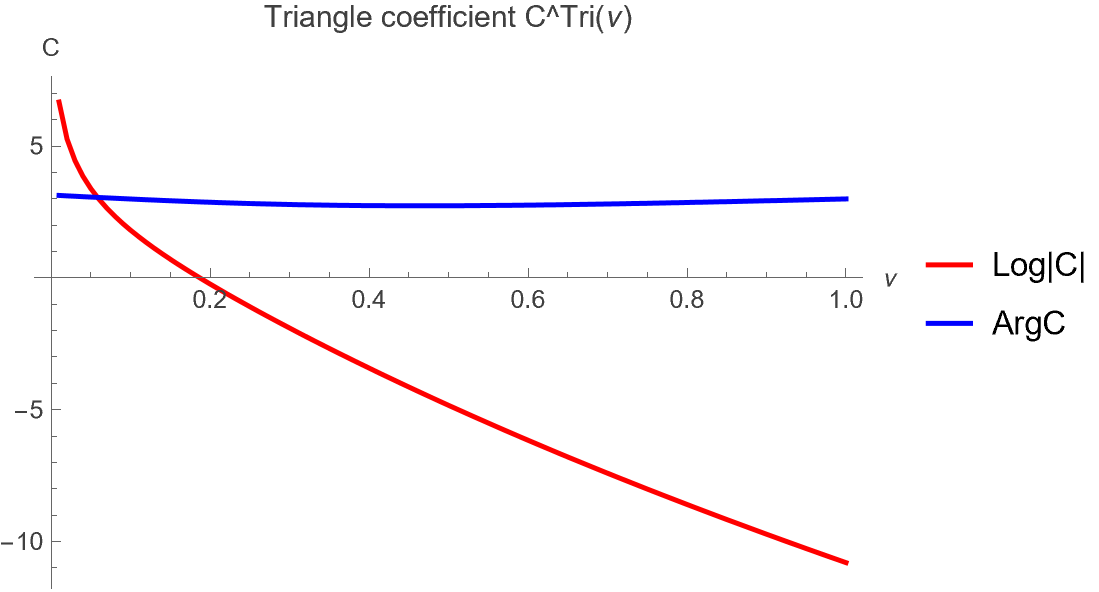
\includegraphics[width=0.80\textwidth]{figure/CTri.png}
    \caption{The coefficient $C_g^{\rm Tri}(\tilde\nu)$  defined in \eqref{eq:triangle-coefficient}.
    The red and blue curves show $\log|C_g^{\rm Tri}|$ and
    $\arg C_g^{\rm Tri}$ in radians, respectively.
    The horizontal variable is $\tilde\nu$.}
    \label{fig:triangle-coefficient}
\end{figure}

\clearpage

\FloatBarrier
\subsection{Box Diagram}
\label{sec:gauge-box}
Now we consider the Higgs trispectrum from the box diagram.
The four cubic vertices give the coupling factor
$(g^2h_0/2)^4=g^8h_0^4/16$, and the diagram symmetry
factor is unity. 

\begin{figure}[htbp]
    \centering
    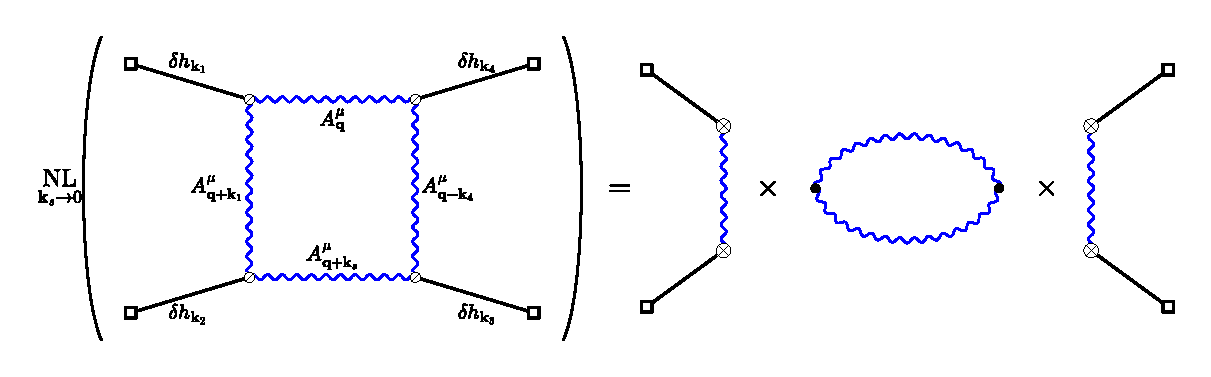
\includegraphics[width=\textwidth]{figure/Box NL.pdf}
    \caption{The leading nonlocal part of the box. Cutting the two soft lines separates
    two tree subgraphs, each containing one hard gauge-boson
    propagator. The central factor contains the nonlocal parts
    of the two soft propagators and their loop momentum integral.}
    \label{fig:box-cutting}
\end{figure}

Choose the loop momenta along the four successive internal lines as
$\mb q+\mb k_1$, $\mb K=\mb q+\mb k_s$, $\mb q-\mb k_4$, and
$\mb q$. In the collapsed limit, the leading nonlocal signal comes
from the region $q,K\sim k_s$. 
Cutting these two soft lines leaves
two hard propagators, with momenta approaching $\mb k_1$ and
$\mb k_3$. 
Their polarizations are denoted by
$\lambda_1,\lambda_3=L,\pm$.
The soft loop gives the dimensionless coefficient
$\mathcal I^{\lambda_1\lambda_3}_{g,\rm Box}
(-\ii\eta\tilde\nu,\theta_1,\theta_3,\phi_3)$ defined in
\eqref{eq:box-I-definition}. 
Its common momentum factor is
$4^{-2\ii\eta\tilde\nu}k_s^{3+4\ii\eta\tilde\nu}$,
as for the bubble and triangle.
As shown in Fig.~\ref{fig:box-cutting}, the time integrals
factorize into two copies of
\eqref{eq:triangle-time-integral}, one for each hard line.
They contribute
$\mathcal P^{(2),\lambda_1}_{g,\eta}(\tilde\nu)$ and
$\mathcal P^{(2),\lambda_3}_{g,\eta}(\tilde\nu)$.
Combining the two branches gives
\begin{align}
    \left[\langle\delta h^4\rangle'_{\mathrm{Box}}
    \right]_{\rm NonL}
    \simeq{}&\frac{g^8h_0^4k_s^3}
    {256k_1^3k_2^3k_3^3k_4^3}
    \left[
    \left(\frac{k_s^2}{4k_{12}k_{34}}\right)^{2\ii\tilde\nu}
    \times
    C_g^{\rm Box}(\tilde\nu,\theta_1,\theta_3,\phi_3)
    +\text{c.c.}\right],
    \label{eq:box-single-signal}
\end{align}
where
\begin{align}
    C_g^{\rm Box}(\tilde\nu,\theta_1,\theta_3,\phi_3)
    ={}&\frac{\Gamma^4(-\ii\tilde\nu)}{(4\pi)^{7/2}}
    \sum_{\lambda_1,\lambda_3=L,\pm}
    \mathcal P^{(2),\lambda_1}_{g,+}(\tilde\nu)
    \mathcal P^{(2),\lambda_3}_{g,+}(\tilde\nu)
    \times\mathcal I^{\lambda_1\lambda_3}_{g,\rm Box}
    (-\ii\tilde\nu,\theta_1,\theta_3,\phi_3).
    \label{eq:box-coefficient}
\end{align}

Since the hard transverse propagators have equal time integrals,
the polarization sum reduces to the $LL$, $LH$, and $HH$ groups
in \eqref{eq:box-channel-groups}. Their explicit expressions are
given in App.~\ref{app:box-coefficients}. In particular,
\eqref{eq:box-C-reduced} shows that all angular dependence is
carried by $\mathcal I^{LL}_{g,\rm Box}$ and multiplied by
$[\mathcal P^{(2),L}_{g,+}-\mathcal P^{(2),+}_{g,+}]^2$.
The difference between the longitudinal and transverse hard-line
time integrals therefore controls the angular dependence of the
box signal.

The result contains five angular structures:
\begin{align}
    C_g^{\rm Box}(\tilde\nu,\theta_1,\theta_3,\phi_3)
    ={}&A_{1,g}(\tilde\nu)
    +A_{2,g}(\tilde\nu)(\cos^2\theta_1+\cos^2\theta_3)
    +A_{3,g}(\tilde\nu)\cos^2\theta_1\cos^2\theta_3
    \nonumber\\
    &+B_g(\tilde\nu)\sin(2\theta_1)\sin(2\theta_3)\cos\phi_3
    \nonumber\\
    &+D_g(\tilde\nu)\sin^2\theta_1\sin^2\theta_3\cos(2\phi_3).
    \label{eq:box-angular-expansion}
\end{align}
The five complex functions depend only on $\tilde\nu$.
The signal is symmetric
under $\theta_1\leftrightarrow\theta_3$ and
$\phi_3\to-\phi_3$. Its oscillatory momentum dependence is the
same as in \eqref{eq:bubble-phase}, with an angle-dependent
amplitude and phase supplied by $C_g^{\rm Box}$.

Figures~\ref{fig:box-A-coefficients} and
\ref{fig:box-BD-coefficients} show the five coefficient functions.
Their magnitudes decrease
over the displayed mass range. The jumps in the plotted phases
reflect the principal branch of $\arg$, defined modulo $2\pi$.

\begin{figure}[p]
    \centering
    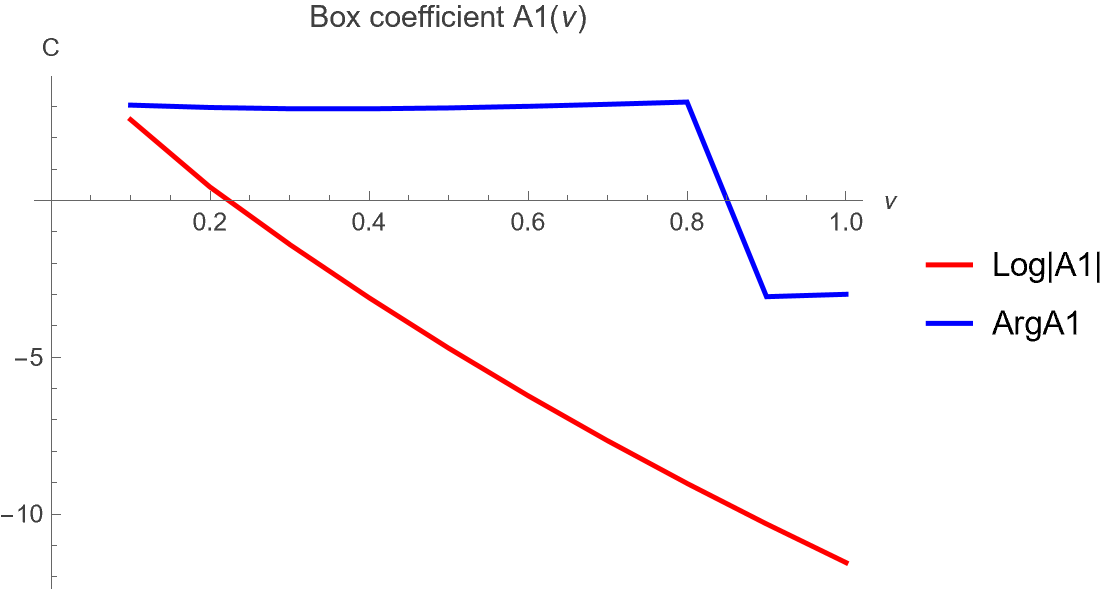
\includegraphics[width=0.70\textwidth]{figure/CBoxA1.png}
    \par\medskip
    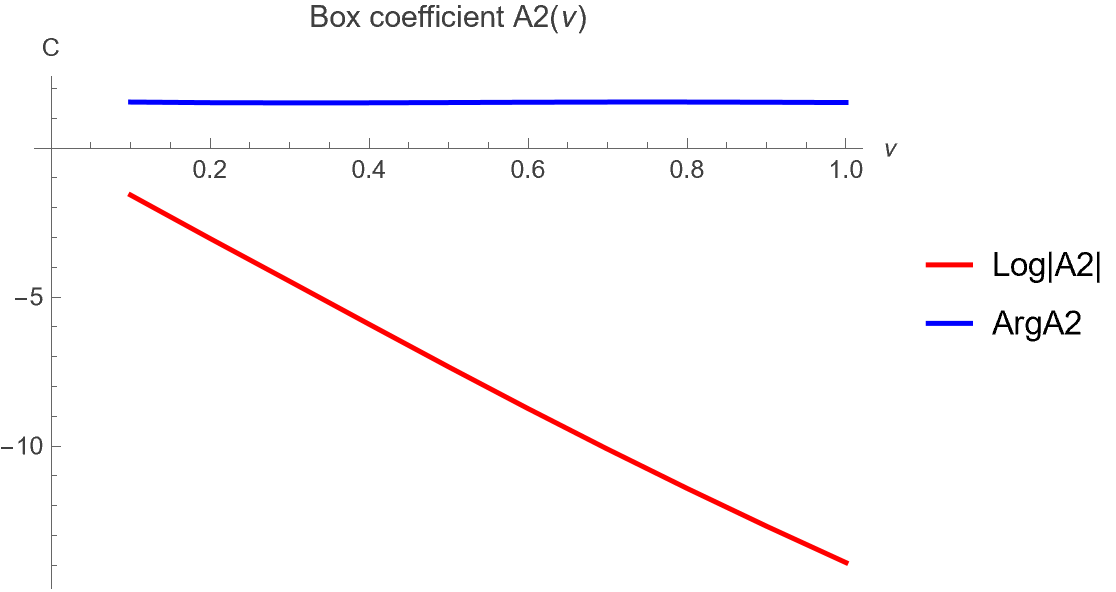
\includegraphics[width=0.70\textwidth]{figure/CBoxA2.png}
    \par\medskip
    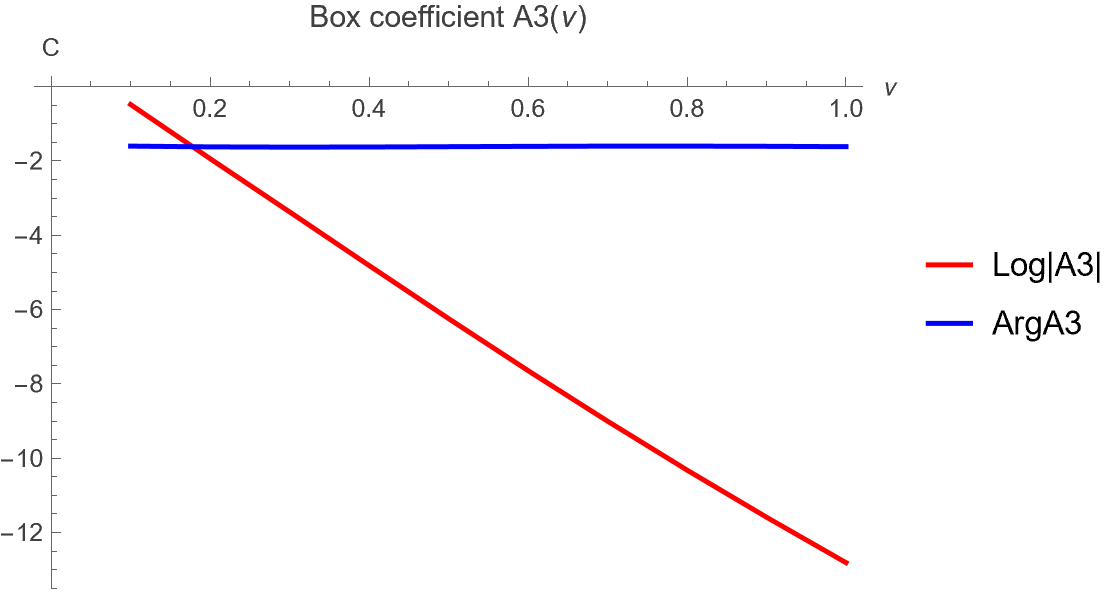
\includegraphics[width=0.70\textwidth]{figure/CBoxA3.png}
    \caption{The angular coefficients $A_{1,g}$, $A_{2,g}$, and $A_{3,g}$
    (top to bottom) in \eqref{eq:box-angular-expansion} for the
    box diagram. Red curves show the logarithmic
    magnitudes and blue curves show the principal phases in radians.
    The horizontal variable is $\tilde\nu$.}
    \label{fig:box-A-coefficients}
\end{figure}

\begin{figure}[p]
    \centering
    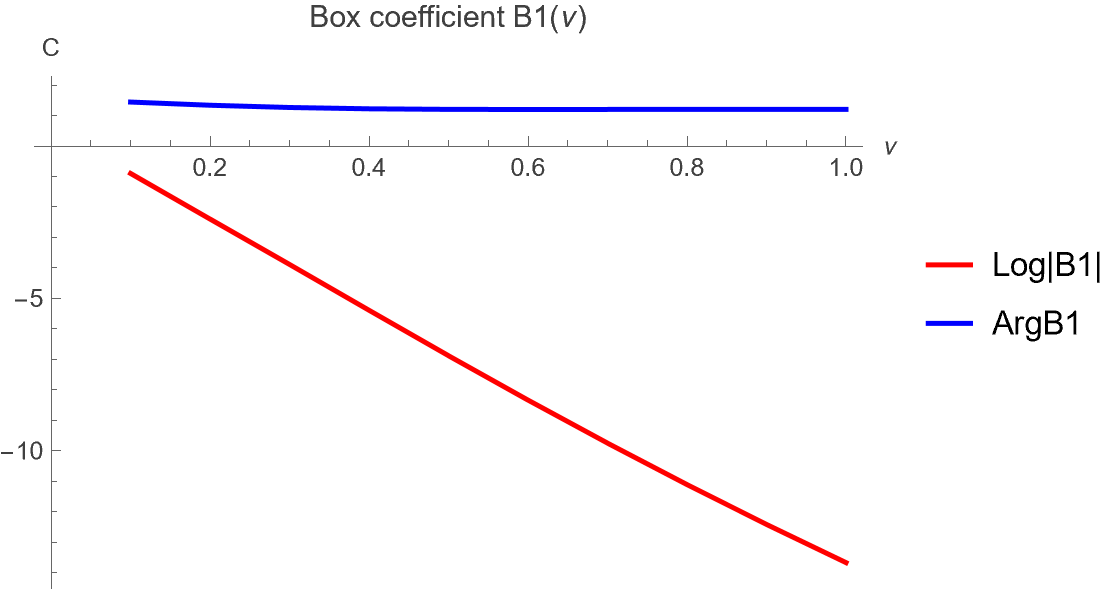
\includegraphics[width=0.80\textwidth]{figure/CBoxB1.png}
    \par\medskip
    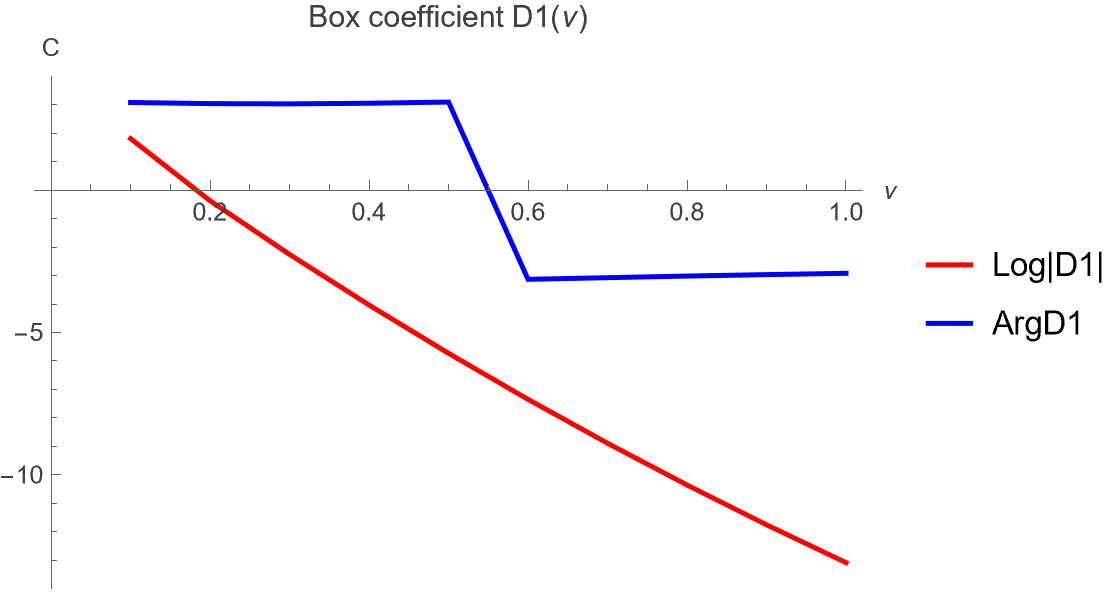
\includegraphics[width=0.80\textwidth]{figure/CBoxD1.png}
    \caption{The angular coefficients $B_g$ (top, labelled $B1$)
    and $D_g$ (bottom, labelled $D1$) in
    \eqref{eq:box-angular-expansion}. The plotting conventions
    are the same as in
    Fig.~\ref{fig:box-A-coefficients}.}
    \label{fig:box-BD-coefficients}
\end{figure}

\clearpage

\section{Top Quark Signal}
\label{sec:top-quark}

\subsection{Preliminaries}
\label{sec:top-preliminaries}
We next compute the Higgs four-point function generated by the top-quark
loop. We use the collapsed kinematics of \eqref{eq:collapsed-kinematics}
and the external propagator \eqref{eq:higgs-propagator}. The top mass is
treated as constant and the chemical potential vanishes. The Yukawa
coupling and mass parameter are
\begin{equation}
 g_t\equiv\frac{y_t}{\sqrt2},\qquad m_t=g_th_0,\qquad
 \tilde\nu\equiv\frac{m_t}{H}>0,\qquad N_c=3.
 \label{eq:top-parameters}
\end{equation}
Thus the relation between $\tilde\nu$ and the mass differs from that
of the vector field. The constant-background approximation requires
$|\dot h_0|\ll H|h_0|$, while the external Higgs modes are evaluated
at $|m_H^2|\ll H^2$ \cite{lu_cosmological_2020}.

Let $t$ and $t^c$ denote the conformally rescaled left-handed top and
the left-handed charge conjugate of the right-handed top. Rescaling
the covariant fields by $a^{3/2}$, with $a=-1/(H\tau)$, gives
\begin{equation}
 \mathcal L=\ii t^\dagger\bar\sigma^\mu\partial_\mu t
 +\ii t^{c\dagger}\bar\sigma^\mu\partial_\mu t^c
 -a(m_t+g_t\delta h)(tt^c+\mathrm{h.c.}).
 \label{eq:top-dirac-action}
\end{equation}
Here $t^c$ represents the right-handed degree of freedom in left-handed
notation. Following the two-component description of
Ref.~\cite{aoki_fermionic_2026}, we set
$t=(\psi_1+\ii\psi_2)/\sqrt2$ and
$t^c=(\psi_1-\ii\psi_2)/\sqrt2$. The action becomes
\begin{equation}
 \mathcal L=\sum_{I=1}^2\left[
 \ii\psi_I^\dagger\bar\sigma^\mu\partial_\mu\psi_I
 -\frac a2(m_t+g_t\delta h)(\psi_I\psi_I+\mathrm{h.c.})\right].
 \label{eq:top-majorana-action}
\end{equation}
The two sectors are identical and independent for the Yukawa loop
considered here. We calculate one sector and restore $2N_c$.
Each vertex retains one factor of $a(\tau)$; the propagators below
are those of the rescaled field and contain no factors of $a^{-3/2}$.

For one sector, the normalized Bunch--Davies modes can be written as
\begin{equation}
 u_+=v_- =\frac{\tilde\nu}{\sqrt{2x}}
 W_{-1/2,\ii\tilde\nu}(-2\ii x),\qquad
 u_-=v_+ =\frac{\ii}{\sqrt{2x}}
 W_{1/2,\ii\tilde\nu}(-2\ii x),\qquad x=-k\tau.
 \label{eq:top-modes}
\end{equation}
The helicity is $s=\pm1$, $|u_s|^2+|v_s|^2=1$, and the creation
part of the field contains $v_s^*$. We use the three propagators
\cite{you_neutrino_2026}
\begin{align}
 D_{\aa\bb,\alpha\dot\beta}(\mb k;\tau_1,\tau_2)
 &=\langle T_C\psi_{\aa,\alpha}(\mb k,\tau_1)
                      \psi^\dagger_{\bb,\dot\beta}(-\mb k,\tau_2)\rangle',
 \nonumber\\
 \widehat D_{\aa\bb,\alpha\beta}(\mb k;\tau_1,\tau_2)
 &=\langle T_C\psi_{\aa,\alpha}(\mb k,\tau_1)
                      \psi_{\bb,\beta}(-\mb k,\tau_2)\rangle',
 \nonumber\\
 \check D_{\aa\bb,\dot\alpha\dot\beta}(\mb k;\tau_1,\tau_2)
 &=\langle T_C\psi^\dagger_{\aa,\dot\alpha}(\mb k,\tau_1)
                      \psi^\dagger_{\bb,\dot\beta}(-\mb k,\tau_2)\rangle'.
 \label{eq:top-propagators}
\end{align}
There is no overall $\ii$ in these definitions. Their mode sums and
fermionic reversal rules are given in App.~\ref{app:top-propagators}.
For each of the three types, the time-ordered components obey
\begin{equation}
 \mathcal D_{++}=\theta_{12}\mathcal D_{-+}+\theta_{21}\mathcal D_{+-},
 \qquad
 \mathcal D_{--}=\theta_{21}\mathcal D_{-+}+\theta_{12}\mathcal D_{+-},
 \qquad \theta_{ij}=\theta(\tau_i-\tau_j).
 \label{eq:top-sk}
\end{equation}
The fermionic exchange sign is included in $\mathcal D_{+-}$.

To display the soft expansion, write
$\sigma_p=\bm\sigma\cdot\widehat{\mb p}$ and
$\epsmat=\ii\sigma^2$, with $\epsilon_{12}=1$ and
$\epsilon^{12}=-1$. Define the common branch coefficient
\begin{equation}
 c_\eta=\frac{2^{-1-2\ii\eta\tilde\nu}}{\pi}
 \Gamma^2(\tfrac12-\ii\eta\tilde\nu),\qquad
 c_-=c_+^*,\qquad |c_+|=\frac1{2\cosh(\pi\tilde\nu)}.
 \label{eq:top-soft-normalization}
\end{equation}
At $|p\tau_1|,|p\tau_2|\ll1$, the required nonlocal terms are
\begin{align}
 [D_{\aa\bb}]_{\rm NonL}
 &=-\frac12\sum_{\eta=\pm1}c_\eta(p^2\tau_1\tau_2)^{\ii\eta\tilde\nu}
 \left[\sigma_p+\frac{\ii p(\tau_1-\tau_2)}{1+2\ii\eta\tilde\nu}\one
 +\cdots\right],\nonumber\\
 [\widehat D_{\aa\bb}]_{\rm NonL}
 &=-\frac12\sum_{\eta=\pm1}\eta c_\eta(p^2\tau_1\tau_2)^{\ii\eta\tilde\nu}
 \left[\sigma_p+\frac{\ii p(\tau_1+\tau_2)}{1+2\ii\eta\tilde\nu}\one
 +\cdots\right]\epsmat,\nonumber\\
 [\check D_{\aa\bb}]_{\rm NonL}
 &=-\frac12\sum_{\eta=\pm1}\eta c_\eta(p^2\tau_1\tau_2)^{\ii\eta\tilde\nu}
 \epsmat\left[\sigma_p-\frac{\ii p(\tau_1+\tau_2)}{1+2\ii\eta\tilde\nu}\one
 +\cdots\right].
 \label{eq:top-soft-propagators}
\end{align}
The omitted terms are second order in the soft momentum at fixed times.
These nonlocal expressions are independent of the SK indices. They
allow the two soft lines to be cut, while the remaining hard lines
retain their full time dependence and SK ordering
\cite{qin_inflation_2023,you_neutrino_2026}.

\subsection{The Box Diagram and Soft Expansion}
\label{sec:top-box}
The Yukawa interaction gives two vertex types, labelled
$r=\mathrm L,\overline{\mathrm L}$ for $\psi\psi$ and
$\psi^\dagger\psi^\dagger$, respectively. Their amputated rules are
$-\ii\aa g_ta(\tau)J_r$, where
$J_{\mathrm L}=\epsmat$ and $J_{\overline{\mathrm L}}=-\epsmat$.
For a fixed ordering $1234$, including both sectors and all colors,
the box is
\begin{align}
 \langle\delta h^4\rangle'_{t,1234}
 ={}&-N_cg_t^4\sum_{\aa_1,\ldots,\aa_4=\pm1}
 \left(\prod_{v=1}^4\aa_v\right)
 \int_{-\infty}^0\prod_{v=1}^4
 [\di\tau_v\,a(\tau_v)G_{\aa_v}(k_v;\tau_v)]\nonumber\\
 &\times\int\frac{\di^3\mb q}{(2\pi)^3}
 \sum_{r_1,\ldots,r_4}
 \tr_2[D_{12}J_{r_2}D_{23}J_{r_3}D_{34}J_{r_4}D_{41}J_{r_1}],
 \label{eq:top-box-integral}
\end{align}
where $D_{ij}=D^{r_ir_j}_{\aa_i\aa_j}(\mb p_{ij};\tau_i,\tau_j)$
and $\tr_2$ contracts the two spinor components. The minus sign is
the closed-fermion-loop sign. A single Majorana sector has the
coefficient $-g_t^4/2$ in this directed-cycle convention; multiplication
by $2N_c$ gives the prefactor in \eqref{eq:top-box-integral}.
The vertex-type sum does not include external permutations.

Choose the successive momenta as $\mb q+\mb k_1$,
$\mb K=\mb q+\mb k_s$, $\mb q-\mb k_4$, and $\mb q$.
In the double-soft region $q,K\sim k_s$, it is useful to introduce
centered hard momenta,
\begin{equation}
 \mb k_L=\frac{\mb k_1-\mb k_2}{2},\qquad
 \mb k_R=\frac{\mb k_3-\mb k_4}{2},\qquad
 \bm\ell=\mb q+\frac{\mb k_s}{2}.
 \label{eq:top-centered-momenta}
\end{equation}
The hard lines then carry $\mb k_L+\bm\ell$ and
$\mb k_R+\bm\ell$. In particular the right momentum is exactly
$\mb q-\mb k_4=\mb q+\mb k_s+\mb k_3$.
At leading collapsed order, $k_L\simeq k_{12}/2$ and
$k_R\simeq k_{34}/2$.

\begin{figure}[htbp]
 \centering
 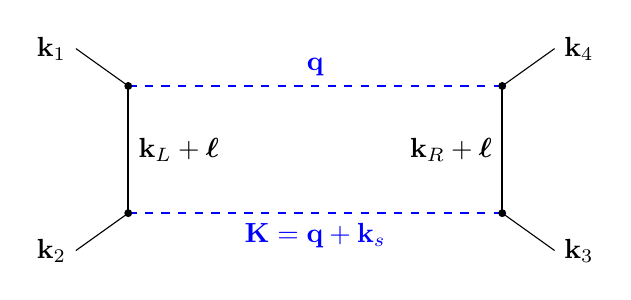
\begin{tikzpicture}[scale=0.95]
  \coordinate (v1) at (0,1.7); \coordinate (v2) at (0,0);
  \coordinate (v3) at (5,0); \coordinate (v4) at (5,1.7);
  \draw[thick,blue,dashed] (v1)--node[above] {$\mb q$} (v4);
  \draw[thick,blue,dashed] (v2)--node[below] {$\mb K=\mb q+\mb k_s$} (v3);
  \draw[thick] (v1)--node[right] {$\mb k_L+\bm\ell$} (v2);
  \draw[thick] (v3)--node[left] {$\mb k_R+\bm\ell$} (v4);
  \draw (v1)--++(-0.7,0.5) node[left] {$\mb k_1$};
  \draw (v2)--++(-0.7,-0.5) node[left] {$\mb k_2$};
  \draw (v3)--++(0.7,-0.5) node[right] {$\mb k_3$};
  \draw (v4)--++(0.7,0.5) node[right] {$\mb k_4$};
  \foreach \i in {1,2,3,4} \fill (v\i) circle (1.5pt);
 \end{tikzpicture}
 \caption{The double-soft region of the top-quark box. Cutting the
 two dashed lines separates the left and right hard exchanges.
 All momentum labels are vectors; the hard propagators retain
 their complete time dependence.}
 \label{fig:top-cut}
\end{figure}

For the same-sign soft branch $\eta=+1$, attaching the soft
endpoints to each hard line gives matrices $V_{12}$ and $V_{34}$.
Their normalization is fixed in App.~\ref{app:top-soft} so that
the cut spin factor of this ordering is
\begin{equation}
 c_+^2(qK)^{2\ii\tilde\nu}\prod_{v=1}^4(-\tau_v)^{\ii\tilde\nu}
 \tr_2[V_{12}\sigma_KV_{34}\sigma_q].
 \label{eq:top-cut-trace}
\end{equation}
The four orderings contributing to the collapsed $s$ channel are
$1234,1243,1342,1432$. They replace the trace by
\begin{equation}
 \tr_2[(V_{12}+V_{21})\sigma_K(V_{34}+V_{43})\sigma_q].
 \label{eq:top-four-orderings}
\end{equation}
Every time and SK label remains attached to its physical external
vertex, so all four terms have the same exact Higgs factors.

At zeroth soft order, the vertex-type sum at a hard end is
proportional to its direction. Writing its scalar coefficient as
$F_{0;\aa\bb}$, one finds
\begin{align}
 V_{12}^{(0)}&=-F_{0;\aa_1\aa_2}(k_L;\tau_1,\tau_2)
                  \bm\sigma\cdot\mb n_L,
 &V_{21}^{(0)}&=+F_{0;\aa_1\aa_2}(k_L;\tau_1,\tau_2)
                  \bm\sigma\cdot\mb n_L,\nonumber\\
 V_{12}^{(0)}+V_{21}^{(0)}&=0,
 &V_{34}^{(0)}+V_{43}^{(0)}&=0,
 \label{eq:top-cancellation}
\end{align}
where $\mb n_L=\widehat{\mb k}_L$ and
$\mb n_R=\widehat{\mb k}_R$. The scalar coefficient is invariant
under reversal of its two time and SK labels. Thus the cancellation
holds before the time integrations or the SK sum. A single ordering
has a nonzero zeroth-order trace, but the sum removes the candidate
$k_s^{3\pm4\ii\tilde\nu}$ oscillatory signal.

The first surviving term has one soft power at each hard end.
Both the magnitude and direction of the hard momentum must be
expanded, together with the first-order soft terms in
\eqref{eq:top-soft-propagators}. Their sum can be organized as
\begin{align}
 V_{12}^{(1)}+V_{21}^{(1)}&=-\frac2{k_L}\bm\sigma\cdot\mb v_L,
 &\mb v_L&=\Pi^L_1\bm\ell+
                  \Pi^L_2\mb n_L(\mb n_L\cdot\bm\ell),\nonumber\\
 V_{34}^{(1)}+V_{43}^{(1)}&=-\frac2{k_R}\bm\sigma\cdot\mb v_R,
 &\mb v_R&=\Pi^R_1\bm\ell+
                  \Pi^R_2\mb n_R(\mb n_R\cdot\bm\ell).
 \label{eq:top-first-order}
\end{align}
The two scalar functions $\Pi_i$ depend on the endpoint times and
SK labels but not on $\mb q$; their explicit expressions are given
in \eqref{eq:top-Pi}. Terms with a zeroth-order end, including the
second-order expansion at the other end, vanish by
\eqref{eq:top-cancellation}. Consequently the first nonzero
oscillatory signal scales as $k_s^{5\pm4\ii\tilde\nu}$.

\subsection{Factorized Loop and Time Integrals}
\label{sec:top-factorized}
The Pauli trace in \eqref{eq:top-four-orderings} reduces the
remaining loop to a scalar integral. We define its dimensionless
coefficients by
\begin{align}
 &\int\frac{\di^3\mb q}{(2\pi)^3}(qK)^{2\ii\tilde\nu-1}
 \left[2(\mb v_L\cdot\bm\ell)(\mb v_R\cdot\bm\ell)
 -\frac12(\mb v_L\cdot\mb k_s)(\mb v_R\cdot\mb k_s)
 -(\mb v_L\cdot\mb v_R)(\ell^2-k_s^2/4)\right]\nonumber\\
 &\hspace{20mm}=k_s^{5+4\ii\tilde\nu}
 \sum_{i,j=1}^2\mathcal I^{ij}_{t,\rm Box}
 (\tilde\nu,\theta_1,\theta_3,\phi_3)\Pi^L_i\Pi^R_j.
 \label{eq:top-loop-definition}
\end{align}
The trace supplies a further factor $8/(k_Lk_R)$, consisting of
$2$ from the Pauli identity and $4$ from the two ordering sums.
At this order the angles of the centered hard directions can be
identified with those in Sec.~\ref{sec:gauge-preliminaries}.
Every polynomial momentum moment in \eqref{eq:top-loop-definition}
reduces to the scalar convolution $f_0$ of \eqref{eq:f0}.
The resulting coefficients satisfy
\begin{equation}
 \mathcal I^{11}_{t,\rm Box}
 =3\mathcal I^{12}_{t,\rm Box}
 =3\mathcal I^{21}_{t,\rm Box}.
 \label{eq:top-loop-relations}
\end{equation}
These three coefficients are independent of angles. All angular
dependence is carried by $\mathcal I^{22}_{t,\rm Box}$, whose
explicit expression is collected in App.~\ref{app:top-soft}.
The integrals are defined by analytic continuation, as in
\eqref{eq:fr-definition}; polynomial contact terms are excluded.

The two time integrations on each side are now independent.
For their leading collapsed values, set the two external energies
equal to the hard magnitude $k$ and define
\begin{align}
 &\frac{4k^6}{H^4}\sum_{\aa,\bb=\pm1}\aa\bb
 \int_{-\infty}^0\di\tau_1\di\tau_2\,
 (-\tau_1)^{\ii\tilde\nu-1}(-\tau_2)^{\ii\tilde\nu-1}
 G_{\aa}(k;\tau_1)G_{\bb}(k;\tau_2)
 \Pi_{i;\aa\bb}(k;\tau_1,\tau_2)
 \nonumber\\
 &\hspace{35mm}=k^{-2\ii\tilde\nu}\mathcal P_{t,i}(\tilde\nu),
 \qquad i=1,2.
 \label{eq:top-time-definition}
\end{align}
The left and right subgraphs use $k=k_L$ and $k=k_R$, respectively.
The coefficient $\mathcal P_{t,1}$ includes the hard-direction
correction and the two soft-endpoint corrections;
$\mathcal P_{t,2}$ contains the hard-magnitude derivative and its
associated direction correction. The exact external propagators
were common factors throughout the cancellation and loop integral.
Corrections to their equal-energy limit enter beyond the leading
nonzero term.

These time integrals reduce to the Whittaker seed of
Ref.~\cite{qin_closed-form_2023}, denoted here by
$\mathcal K_{\aa\bb}^{\kappa;p_1p_2}$ with $\kappa=\pm1/2$.
This plays the same role for $\mathcal P_{t,i}$ as
$\mathcal M_{\aa\bb}^{p_1p_2}$ does for the gauge-boson coefficients.
Its scalar kernel has a different normalization from
$D^{\rm(s)}$ in \eqref{eq:scalar-propagator}.
The continuation in $\kappa$ is an auxiliary method of evaluating
the fermion modes; the physical top chemical potential remains zero.
The seed normalization, its closed form and the combinations giving
$\mathcal P_{t,i}$ are given in App.~\ref{app:top-seed}.
A common endpoint regulator is removed after the complete SK sum
has been assembled.

\subsection{Oscillatory Signal}
\label{sec:top-clock}
Combining the soft loop and the two hard subgraphs, and adding the
complex-conjugate branch, gives
\begin{align}
 \left[\langle\delta h^4\rangle'_{t,s}\right]_{\rm osc}
 \simeq{}&-\frac{N_cg_t^4H^4k_s^5}
 {16k_1^3k_2^3k_3^3k_4^3k_Lk_R}\nonumber\\
 &\times\left[
 \left(\frac{k_s^2}{4k_{12}k_{34}}\right)^{2\ii\tilde\nu}
 C_t^{\rm Box}(\tilde\nu,\theta_1,\theta_3,\phi_3)
 +\text{c.c.}\right],
 \label{eq:top-clock-signal}
\end{align}
where
\begin{equation}
 C_t^{\rm Box}
 =8c_+^2\,16^{2\ii\tilde\nu}
 \sum_{i,j=1}^2\mathcal P_{t,i}\mathcal P_{t,j}
                    \mathcal I^{ij}_{t,\rm Box}.
 \label{eq:top-clock-coefficient}
\end{equation}
All four $s$-channel orderings are included. The phase factor
$16^{2\ii\tilde\nu}$ converts the natural hard scale $k_Lk_R$
to the momentum ratio used in Sec.~\ref{sec:gauge-boson}, since
$4k_{12}k_{34}\simeq16k_Lk_R$.

The angular decomposition takes the same form as
\eqref{eq:box-angular-expansion}:
\begin{align}
 C_t^{\rm Box}={}&A_{1,t}
 +A_{2,t}(\cos^2\theta_1+\cos^2\theta_3)
 +A_{3,t}\cos^2\theta_1\cos^2\theta_3\nonumber\\
 &+B_t\sin(2\theta_1)\sin(2\theta_3)\cos\phi_3
 +D_t\sin^2\theta_1\sin^2\theta_3\cos(2\phi_3).
 \label{eq:top-angular}
\end{align}
The five coefficients depend only on $\tilde\nu$ and satisfy
$A_{3,t}=-3A_{2,t}$. Their analytic expressions are given in
App.~\ref{app:top-coefficients}. In particular all nonconstant
angular terms are proportional to $\mathcal P_{t,2}^2$.
The result is even under either Higgs-pair exchange and under parity.

At fixed angles the oscillatory bracket in
\eqref{eq:top-clock-signal} is
\begin{equation}
 2|C_t^{\rm Box}|\cos\left[
 2\tilde\nu\log\!\left(\frac{k_s^2}{4k_{12}k_{34}}\right)
 +\arg C_t^{\rm Box}\right].
 \label{eq:top-clock-phase}
\end{equation}
The frequency in $\log k_s$ is $4m_t/H$.
Compared with the gauge-boson signals, the top oscillation carries
an additional soft suppression $k_s^2/(k_Lk_R)$ from
\eqref{eq:top-cancellation}. The coefficient determines its
mass-dependent and angle-dependent amplitude and phase.

\subsection{Nonoscillatory Signal}
\label{sec:top-mixed}
Opposite branches on the two cut lines produce a nonoscillatory
contribution. Their zeroth-order hard matrices are proportional
to $\one$, with scalar coefficient $F_1$ defined in
App.~\ref{app:top-propagators}. They are even under the external
exchange and therefore survive the ordering sum. The spin trace
is proportional to $2\widehat{\mb q}\cdot\widehat{\mb K}$.
The corresponding soft convolution is
\begin{equation}
 \int\frac{\di^3\mb q}{(2\pi)^3}
 (q^2)^{-\ii\tilde\nu}(K^2)^{\ii\tilde\nu}
 \widehat{\mb q}\cdot\widehat{\mb K}
 =\frac{k_s^3}{(4\pi)^{3/2}}
 \frac{2\sqrt\pi}{3}\tilde\nu(1+\tilde\nu^2)
 \coth(\pi\tilde\nu).
 \label{eq:top-mixed-loop}
\end{equation}
Both hard subgraphs give the same real time coefficient
$\mathcal P_{t,\rm mix}$, evaluated through $\mathcal K$ in
\eqref{eq:top-P-from-seed}. Summing the two opposite-branch
assignments and the four orderings yields
\begin{equation}
 \left[\langle\delta h^4\rangle'_{t,s}\right]_{\rm mix}
 \simeq\frac{N_cg_t^4H^4k_s^3}{16k_1^3k_2^3k_3^3k_4^3}
 \frac{2\tilde\nu(1+\tilde\nu^2)}{3\pi\sinh(2\pi\tilde\nu)}
 \mathcal P_{t,\rm mix}^2.
 \label{eq:top-mixed-signal}
\end{equation}
This term has no angular dependence at leading order.
Although it does not oscillate, $k_s^3=(\mb k_s^2)^{3/2}$ is
nonanalytic in the soft momentum components and is not a
polynomial contact contribution.

Equations~\eqref{eq:top-clock-signal} and \eqref{eq:top-mixed-signal}
give the leading oscillatory and nonoscillatory nonanalytic terms,
respectively, for fixed $\tilde\nu>0$ in one collapsed channel.
The coincident branches at $\tilde\nu=0$ require a combined limit.
Analytic contact terms and the conversion of Higgs fluctuations
into curvature perturbations are not included.


\section{Conclusions}
\label{sec:conclusions}
% Intentionally left blank.

\appendix
\section{Gauge Boson Integrals and Coefficients}
\label{app:gauge}
\subsection{Loop Integral Formulae}
\label{app:appendix}
\label{app:loop-integrals}
The identity $z=(K^2-q^2-k_s^2)/(2qk_s)$ reduces all angular moments
in \eqref{eq:fr-definition} to the scalar integral $f_0$:
\begin{equation}
    f_r(\alpha,\beta)=\frac1{2^r}
    \sum_{u+v+w=r}\frac{r!}{u!v!w!}(-1)^{v+w}
    f_0\left(\alpha+\frac r2-v,\beta-u\right),
    \label{eq:fr-finite-sum}
\end{equation}
where the sum runs over nonnegative integers. For the third and fourth
moments this gives
\begin{align}
    f_3(\alpha,\beta)=\frac18\Big[&
    f_0(\alpha+\tfrac32,\beta-3)
    -3f_0(\alpha+\tfrac32,\beta-2)
    -3f_0(\alpha+\tfrac12,\beta-2)\nonumber\\
    &+3f_0(\alpha+\tfrac32,\beta-1)
    +6f_0(\alpha+\tfrac12,\beta-1)
    +3f_0(\alpha-\tfrac12,\beta-1)\nonumber\\
    &-f_0(\alpha+\tfrac32,\beta)
    -3f_0(\alpha+\tfrac12,\beta)
    -3f_0(\alpha-\tfrac12,\beta)
    -f_0(\alpha-\tfrac32,\beta)\Big],
    \label{eq:f3}\\[1mm]
    f_4(\alpha,\beta)=\frac1{16}\Big[&
    f_0(\alpha+2,\beta-4)
    -4f_0(\alpha+2,\beta-3)-4f_0(\alpha+1,\beta-3)\nonumber\\
    &+6f_0(\alpha+2,\beta-2)+12f_0(\alpha+1,\beta-2)
    +6f_0(\alpha,\beta-2)\nonumber\\
    &-4f_0(\alpha+2,\beta-1)-12f_0(\alpha+1,\beta-1)
    -12f_0(\alpha,\beta-1)\nonumber\\
    &-4f_0(\alpha-1,\beta-1)
    +f_0(\alpha+2,\beta)+4f_0(\alpha+1,\beta)\nonumber\\
    &+6f_0(\alpha,\beta)+4f_0(\alpha-1,\beta)
    +f_0(\alpha-2,\beta)\Big].
    \label{eq:f4}
\end{align}

\subsection{Bubble Coefficients}
\label{app:bubble-polarizations}
For $x=-\ii\eta\tilde\nu$, the relative weight of a longitudinal
nonlocal propagator is
\begin{equation}
    \beta(x)\equiv\frac{(x+1/2)^2}{1/4-x^2}
    =\frac{1+2x}{1-2x}.
    \label{eq:bubble-longitudinal-weight}
\end{equation}
Define $\mathcal I_{g,\sigma_1\sigma_2}(x)$ by restricting the loop in
\eqref{eq:bubble-cut-loop} to the polarizations
$(\sigma_1,\sigma_2)$ and replacing $\mathcal I_{g,\rm Bub}$ on its
right-hand side by $\mathcal I_{g,\sigma_1\sigma_2}$. The independent
coefficients are
\begin{align}
    \mathcal I_{g,LL}(x)
    &=[\beta(x)]^2
    \left[\mathcal J_0(2,2;x)+2\mathcal J_1(1,2;x)
    +\mathcal J_2(0,2;x)\right],
    \label{eq:bubble-ILL}\\
    \mathcal I_{g,L+}(x)
    &=\frac{\beta(x)}2
    \left[\mathcal J_0(0,2;x)-\mathcal J_2(0,2;x)\right],
    \label{eq:bubble-ILplus}\\
    \mathcal I_{g,++}(x)
    &=\frac14\left[
    \mathcal J_0(0,0;x)+\mathcal J_0(2,2;x)
    +\mathcal J_2(0,2;x)\right.\nonumber\\
    &\hspace{12mm}\left.
    +2\mathcal J_0(1,1;x)+2\mathcal J_1(1,2;x)
    +2\mathcal J_1(0,1;x)\right],
    \label{eq:bubble-Iplusplus}\\
    \mathcal I_{g,+-}(x)
    &=\frac14\left[
    \mathcal J_0(0,0;x)+\mathcal J_0(2,2;x)
    +\mathcal J_2(0,2;x)\right.\nonumber\\
    &\hspace{12mm}\left.
    -2\mathcal J_0(1,1;x)+2\mathcal J_1(1,2;x)
    -2\mathcal J_1(0,1;x)\right].
    \label{eq:bubble-Iplusminus}
\end{align}
The remaining entries satisfy
$\mathcal I_{g,--}=\mathcal I_{g,++}$,
$\mathcal I_{g,-+}=\mathcal I_{g,+-}$, and
$\mathcal I_{g,L-}=\mathcal I_{g,+L}=\mathcal I_{g,-L}=\mathcal I_{g,L+}$.
Consequently,
\begin{equation}
    \mathcal I_{g,\rm Bub}
    =\mathcal I_{g,LL}+4\mathcal I_{g,L+}
    +2\mathcal I_{g,++}+2\mathcal I_{g,+-},
    \label{eq:bubble-channel-sum}
\end{equation}
which reduces to \eqref{eq:bubble-polarization-sum} using the moment
relations in App.~\ref{app:loop-integrals}.

For the $\eta=+1$ branch, the fully reduced sum is
\begin{equation}
    \mathcal I_{g,\rm Bub}(-\ii\tilde\nu)
    =\frac{3\cdot2^{-4-4\ii\tilde\nu}(3\ii-2\tilde\nu)^2
    \Gamma(-3/2-2\ii\tilde\nu)\Gamma(3+2\ii\tilde\nu)
    \sinh^2(\pi\tilde\nu)}
    {\pi[1+(3\ii-2\tilde\nu)\tilde\nu]^2}.
    \label{eq:bubble-I-closed}
\end{equation}
Substituting this into \eqref{eq:bubble-coefficient} gives
\begin{align}
    C_g^{\rm Bub}(\tilde\nu)
    ={}&\frac{3(\tilde\nu-\ii)(\tilde\nu-2\ii)^4}
    {256\pi^{7/2}\tilde\nu^2(2\tilde\nu-\ii)}
    \Gamma^2(-2-\ii\tilde\nu)\Gamma^2(5/2+\ii\tilde\nu)
    \nonumber\\
    &\times\Gamma(-3/2-2\ii\tilde\nu)
    \Gamma(1+2\ii\tilde\nu)\sinh^2(\pi\tilde\nu).
    \label{eq:bubble-C-closed}
\end{align}
For real
$\tilde\nu>0$, the opposite nonlocal branch is their complex conjugate.

\subsection{Triangle Coefficients}
\label{app:triangle-coefficients}
\subsubsection{Polarization sum}
Let $x=-\ii\eta\tilde\nu$ and let $\beta(x)$ be the longitudinal
weight in \eqref{eq:bubble-longitudinal-weight}. Summing the nine
soft-polarization combinations gives
\begin{align}
    \mathcal I^L_{g,\rm Tri}(x,\theta)
    ={}&[\beta(x)]^2\left\{
    \frac{\sin^2\theta}{2}\left[
    \mathcal J_0(2,2;x)+\mathcal J_1(1,2;x)
    -\mathcal J_2(2,2;x)-\mathcal J_3(1,2;x)\right]\right.
    \nonumber\\
    &\hspace{15mm}\left.+\cos^2\theta\left[
    \mathcal J_2(2,2;x)+\mathcal J_3(1,2;x)
    +\mathcal J_1(1,2;x)+\mathcal J_2(0,2;x)\right]\right\}
    \nonumber\\
    &+\frac{\beta(x)(1+\cos^2\theta)}2
    \left[\mathcal J_0(0,2;x)-\mathcal J_2(0,2;x)\right]
    \nonumber\\
    &+\frac{\sin^2\theta}{2}\left[
    \mathcal J_2(2,2;x)+\mathcal J_3(1,2;x)
    +\mathcal J_1(1,2;x)+\mathcal J_2(0,2;x)
    +\mathcal J_0(0,0;x)\right]
    \nonumber\\
    &+\cos^2\theta\left[
    \mathcal J_0(2,2;x)-\mathcal J_2(2,2;x)
    +\mathcal J_1(1,2;x)-\mathcal J_3(1,2;x)\right].
    \label{eq:triangle-IL-explicit}
\end{align}
The terms proportional to $\beta^2$, $\beta$, and $1$ arise from
two longitudinal, mixed, and two transverse soft lines, respectively.

For a hard line with helicity $+$, the corresponding expression is
\begin{align}
    \mathcal I^+_{g,\rm Tri}(x,\theta)
    ={}&[\beta(x)]^2\left\{
    \frac{1+\cos^2\theta}{4}\left[
    \mathcal J_0(2,2;x)-\mathcal J_2(2,2;x)
    +\mathcal J_1(1,2;x)-\mathcal J_3(1,2;x)\right]\right.
    \nonumber\\
    &\hspace{15mm}\left.+\frac{\sin^2\theta}{2}\left[
    \mathcal J_2(2,2;x)+\mathcal J_1(1,2;x)
    +\mathcal J_3(1,2;x)+\mathcal J_2(0,2;x)\right]\right\}
    \nonumber\\
    &+\frac{\beta(x)(2+\sin^2\theta)}4
    \left[\mathcal J_0(0,2;x)-\mathcal J_2(0,2;x)\right]
    \nonumber\\
    &+\frac{1+\cos^2\theta}{4}\left[
    \mathcal J_2(2,2;x)+\mathcal J_1(1,2;x)
    +\mathcal J_3(1,2;x)+\mathcal J_2(0,2;x)
    +\mathcal J_0(0,0;x)\right]
    \nonumber\\
    &+\frac{\sin^2\theta}{2}\left[
    \mathcal J_0(2,2;x)-\mathcal J_2(2,2;x)
    +\mathcal J_1(1,2;x)-\mathcal J_3(1,2;x)\right].
    \label{eq:triangle-IP-explicit}
\end{align}
At zero chemical potential, reducing the Gamma functions gives the same
result for all three hard-line polarizations:
\begin{align}
    \mathcal I^L_{g,\rm Tri}(-\ii\tilde\nu,\theta)
    &=\mathcal I^+_{g,\rm Tri}(-\ii\tilde\nu,\theta)
    =\mathcal I^-_{g,\rm Tri}(-\ii\tilde\nu,\theta)
    =\frac13\mathcal I_{g,\rm Bub}(-\ii\tilde\nu)
    \nonumber\\
    &=\frac{2^{-4-4\ii\tilde\nu}(3\ii-2\tilde\nu)^2
    \Gamma(-3/2-2\ii\tilde\nu)\Gamma(3+2\ii\tilde\nu)
    \sinh^2(\pi\tilde\nu)}
    {\pi[1+(3\ii-2\tilde\nu)\tilde\nu]^2}.
    \label{eq:triangle-I-closed}
\end{align}
Summing over the hard-line polarizations reproduces
$\mathcal I_{g,\rm Bub}$ by polarization completeness.
Thus the angular dependence of the separate soft-polarization
contributions cancels in their sum. The coefficient of a single
triangle reduces to
\begin{equation}
    C_g^{\rm Tri}(\tilde\nu)
    =\frac{\Gamma^4(-\ii\tilde\nu)}{3(4\pi)^{7/2}}
    \mathcal P^{(1)}_{g,+}(\tilde\nu)
    \left[\mathcal P^{(2),L}_{g,+}(\tilde\nu)
    +2\mathcal P^{(2),+}_{g,+}(\tilde\nu)\right]
    \mathcal I_{g,\rm Bub}(-\ii\tilde\nu).
    \label{eq:triangle-C-reduced}
\end{equation}

\subsubsection{Time-integral coefficients}
For the scalar propagator of \eqref{eq:scalar-propagator},
the double-folded seed is defined by
\begin{equation}
    \mathcal M_{\aa\bb}^{p_1p_2}
    \equiv(-\aa\bb)k^{5+p_{12}}
    \int_{-\infty}^0\di\tau_1\di\tau_2\,
    (-\tau_1)^{p_1}(-\tau_2)^{p_2}
    e^{\ii\aa k\tau_1+\ii\bb k\tau_2}
    \frac{D^{\rm(s)}_{\aa\bb}(k;\tau_1,\tau_2)}{H^2},
    \label{eq:triangle-M-definition}
\end{equation}
This is the seed $\widetilde{\mathcal I}_{\aa\bb}^{p_1p_2}(1,1)$
of Ref.~\cite{qin_closed-form_2023}, with $H$ restored explicitly.
All seeds below have mass index $\tilde\nu$.
The closed expressions are
\begin{align}
    \mathcal M_{\pm\mp}^{p_1p_2}
    &=\frac{e^{\mp\ii\pi\bar p_{12}/2}}{2^{5+p_{12}}}
    \prod_{j=1}^{2}
    \frac{\Gamma(5/2+p_j-\ii\tilde\nu)
    \Gamma(5/2+p_j+\ii\tilde\nu)}{\Gamma(3+p_j)},
    \label{eq:triangle-M-opposite}\\
    \mathcal M_{\pm\pm}^{p_1p_2}
    &=\frac{\pm\ii e^{\mp\ii\pi p_{12}/2}e^{-\pi\tilde\nu}}
    {2^{5+p_{12}}}
    \prod_{j=1}^{2}
    \frac{\Gamma(5/2+p_j-\ii\tilde\nu)
    \Gamma(5/2+p_j+\ii\tilde\nu)}{\Gamma(3+p_j)}
    \nonumber\\
    &\quad-\frac{e^{\mp\ii\pi p_{12}/2}}{2^{5+p_{12}}}
    \Gamma(5+p_{12})\Gamma(5/2+p_1\pm\ii\tilde\nu)
    \Gamma(5/2+p_2\pm\ii\tilde\nu)
    \nonumber\\
    &\qquad\times{}_3\widetilde F_2\left[
    \begin{matrix}
    5+p_{12},\;1/2\pm\ii\tilde\nu,\;1\\
    7/2+p_1\pm\ii\tilde\nu,\;7/2+p_2\pm\ii\tilde\nu
    \end{matrix}\middle|1\right].
    \label{eq:triangle-M-same}
\end{align}
Here ${}_3\widetilde F_2(a,b,c;d,e;1)
={}_3F_2(a,b,c;d,e;1)/[\Gamma(d)\Gamma(e)]$ is the regularized
hypergeometric function.

Set $p_\epsilon=-5/2+\epsilon+\ii\eta\tilde\nu$.
The two transverse coefficients are
\begin{align}
    \mathcal P^{(2),\pm}_{g,\eta}(\tilde\nu)
    ={}&2^{2\ii\eta\tilde\nu}
    \underset{\epsilon=0}{\operatorname{FP}}
    \sum_{\aa,\bb=\pm1}
    \left[
    \mathcal M_{\aa\bb}^{p_\epsilon,p_\epsilon}
    +\ii\aa\mathcal M_{\aa\bb}^{p_\epsilon+1,p_\epsilon}
    +\ii\bb\mathcal M_{\aa\bb}^{p_\epsilon,p_\epsilon+1}
    -\aa\bb\mathcal M_{\aa\bb}^{p_\epsilon+1,p_\epsilon+1}
    \right].
    \label{eq:triangle-P2-transverse}
\end{align}
The longitudinal coefficient can be written using the same transverse
combination:
\begin{align}
    \mathcal P^{(2),L}_{g,\eta}(\tilde\nu)
    ={}&\frac{\mathcal P^{(1)}_{g,\eta}(\tilde\nu)
    +(1/2+\ii\eta\tilde\nu)^2
    \mathcal P^{(2),+}_{g,\eta}(\tilde\nu)}{\tilde\nu^2+1/4}
    \nonumber\\
    &+\frac{2^{2\ii\eta\tilde\nu}}{\tilde\nu^2+1/4}
    \underset{\epsilon=0}{\operatorname{FP}}
    \sum_{\aa,\bb=\pm1}
    \left\{(1/2+\ii\eta\tilde\nu)
    \left[
    \mathcal M_{\aa\bb}^{p_\epsilon+2,p_\epsilon}
    +\ii\bb\mathcal M_{\aa\bb}^{p_\epsilon+2,p_\epsilon+1}
    \right.\right.\nonumber\\
    &\hspace{30mm}\left.\left.
    +\mathcal M_{\aa\bb}^{p_\epsilon,p_\epsilon+2}
    +\ii\aa\mathcal M_{\aa\bb}^{p_\epsilon+1,p_\epsilon+2}
    \right]
    +\mathcal M_{\aa\bb}^{p_\epsilon+2,p_\epsilon+2}
    \right\}.
    \label{eq:triangle-P2-longitudinal}
\end{align}
The operator $\operatorname{FP}_{\epsilon=0}$ selects the constant
coefficient of the Laurent expansion after assembling the indicated
seed sum. In particular, the seed expressions are combined before
setting $\epsilon$ to zero. The first term proportional to
$\mathcal P^{(1)}_{g,\eta}$ in \eqref{eq:triangle-P2-longitudinal} is
the contact contribution from differentiating the time-ordering
step functions.

\subsection{Box Coefficients}
\label{app:box-coefficients}
\subsubsection{Polarization sums}
Let $\lambda_1,\lambda_3=L,\pm$ denote the polarizations of the
hard lines with momenta $\mb k_1$ and $\mb k_3$. With
$\mb K=\mb q+\mb k_s$, define the soft-polarization sum by
\begin{align}
    &\sum_{\sigma_1,\sigma_2=L,\pm}
    [\beta(x)]^{\delta_{\sigma_1L}+\delta_{\sigma_2L}}
    \int\frac{\di^3\mb q}{(2\pi)^3}
    \left(\frac q2\right)^{-2x}
    \left(\frac K2\right)^{-2x}
    (e_{\mb k_1}^{(\lambda_1)*}\!\cdot e_{\mb K}^{(\sigma_1)})
    (e_{\mb K}^{(\sigma_1)*}\!\cdot e_{\mb k_3}^{(\lambda_3)})
    \nonumber\\
    &\qquad\times
    (e_{\mb k_3}^{(\lambda_3)*}\!\cdot e_{\mb q}^{(\sigma_2)})
    (e_{\mb q}^{(\sigma_2)*}\!\cdot e_{\mb k_1}^{(\lambda_1)})
    =\frac{4^{2x}k_s^{3-4x}}{(4\pi)^{3/2}}
    \mathcal I^{\lambda_1\lambda_3}_{g,\rm Box}
    (x,\theta_1,\theta_3,\phi_3).
    \label{eq:box-I-definition}
\end{align}
The angles are defined by the convention stated below
\eqref{eq:collapsed-kinematics}. The two transverse hard-line coefficients
$\mathcal P^{(2),+}_{g,\eta}=\mathcal P^{(2),-}_{g,\eta}$ are equal, so it
suffices to retain three groups:
\begin{align}
    \mathcal I^{LH}_{g,\rm Box}
    &\equiv\sum_{\lambda=\pm}
    \left(\mathcal I^{L\lambda}_{g,\rm Box}
    +\mathcal I^{\lambda L}_{g,\rm Box}\right),
    &\mathcal I^{HH}_{g,\rm Box}
    &\equiv\sum_{\lambda_1,\lambda_3=\pm}
    \mathcal I^{\lambda_1\lambda_3}_{g,\rm Box},
    \label{eq:box-channel-groups}
\end{align}
together with $\mathcal I^{LL}_{g,\rm Box}$. Here $H$ in a polarization
superscript denotes the sum over transverse helicities.

For $x=-\ii\tilde\nu$, the longitudinal result is
\begin{align}
    &\mathcal I^{LL}_{g,\rm Box}
    (-\ii\tilde\nu,\theta_1,\theta_3,\phi_3)
    \nonumber\\
    &\quad=-\frac{4^{-3-2\ii\tilde\nu}(2\tilde\nu-3\ii)
    \Gamma(-3/2-2\ii\tilde\nu)\Gamma(1+2\ii\tilde\nu)
    \sinh^2(\pi\tilde\nu)}
    {\pi(\tilde\nu-\ii)(\tilde\nu-2\ii)(2\tilde\nu-\ii)}
    \nonumber\\
    &\qquad\times\Big\{
    -16-19\ii\tilde\nu+6\tilde\nu^2
    +\tilde\nu(2\tilde\nu-\ii)
    \big[\cos(2\theta_1)+\cos(2\theta_3)
    +3\cos(2\theta_1)\cos(2\theta_3)\big]
    \nonumber\\
    &\hspace{24mm}
    +4(2\tilde\nu^2-5\ii\tilde\nu-3)
    \cos(2\phi_3)\sin^2\theta_1\sin^2\theta_3
    \nonumber\\
    &\hspace{24mm}
    -8\tilde\nu(\tilde\nu-\ii)\cos\phi_3
    \sin(2\theta_1)\sin(2\theta_3)\Big\}.
    \label{eq:box-ILL-closed}
\end{align}
Reducing the mixed and transverse results to the same Gamma-function
basis gives
\begin{align}
    &\mathcal I^{LH}_{g,\rm Box}
    (-\ii\tilde\nu,\theta_1,\theta_3,\phi_3)
    \nonumber\\
    &\quad=-\frac{2\cdot4^{-3-2\ii\tilde\nu}(2\tilde\nu-3\ii)
    \Gamma(-3/2-2\ii\tilde\nu)\Gamma(1+2\ii\tilde\nu)
    \sinh^2(\pi\tilde\nu)}
    {\pi(\tilde\nu-\ii)(\tilde\nu-2\ii)(2\tilde\nu-\ii)}
    \nonumber\\
    &\qquad\times\Big\{
    -32-37\ii\tilde\nu+10\tilde\nu^2
    -\tilde\nu(2\tilde\nu-\ii)
    \big[\cos(2\theta_1)+\cos(2\theta_3)
    +3\cos(2\theta_1)\cos(2\theta_3)\big]
    \nonumber\\
    &\hspace{24mm}
    -4(2\tilde\nu^2-5\ii\tilde\nu-3)
    \cos(2\phi_3)\sin^2\theta_1\sin^2\theta_3
    \nonumber\\
    &\hspace{24mm}
    +8\tilde\nu(\tilde\nu-\ii)\cos\phi_3
    \sin(2\theta_1)\sin(2\theta_3)\Big\},
    \label{eq:box-ILH-explicit}\\[1ex]
    &\mathcal I^{HH}_{g,\rm Box}
    (-\ii\tilde\nu,\theta_1,\theta_3,\phi_3)
    \nonumber\\
    &\quad=-\frac{4^{-3-2\ii\tilde\nu}(2\tilde\nu-3\ii)
    \Gamma(-3/2-2\ii\tilde\nu)\Gamma(1+2\ii\tilde\nu)
    \sinh^2(\pi\tilde\nu)}
    {\pi(\tilde\nu-\ii)(\tilde\nu-2\ii)(2\tilde\nu-\ii)}
    \nonumber\\
    &\qquad\times\Big\{
    -64-75\ii\tilde\nu+22\tilde\nu^2
    +\tilde\nu(2\tilde\nu-\ii)
    \big[\cos(2\theta_1)+\cos(2\theta_3)
    +3\cos(2\theta_1)\cos(2\theta_3)\big]
    \nonumber\\
    &\hspace{24mm}
    +4(2\tilde\nu^2-5\ii\tilde\nu-3)
    \cos(2\phi_3)\sin^2\theta_1\sin^2\theta_3
    \nonumber\\
    &\hspace{24mm}
    -8\tilde\nu(\tilde\nu-\ii)\cos\phi_3
    \sin(2\theta_1)\sin(2\theta_3)\Big\}.
    \label{eq:box-IHH-explicit}
\end{align}
These expressions satisfy the relations implied by polarization
completeness and \eqref{eq:triangle-I-closed}:
\begin{align}
    \mathcal I^{LH}_{g,\rm Box}
    &=\frac23\mathcal I_{g,\rm Bub}-2\mathcal I^{LL}_{g,\rm Box},
    \label{eq:box-ILH-closed}\\
    \mathcal I^{HH}_{g,\rm Box}
    &=\frac13\mathcal I_{g,\rm Bub}+\mathcal I^{LL}_{g,\rm Box}.
    \label{eq:box-IHH-closed}
\end{align}
Indeed, all angular terms cancel in
$\mathcal I^{LH}_{g,\rm Box}+2\mathcal I^{LL}_{g,\rm Box}$ and
$\mathcal I^{HH}_{g,\rm Box}-\mathcal I^{LL}_{g,\rm Box}$.
The three groups therefore also satisfy
$\mathcal I^{LL}_{g,\rm Box}+\mathcal I^{LH}_{g,\rm Box}
+\mathcal I^{HH}_{g,\rm Box}=\mathcal I_{g,\rm Bub}$.

The dimensionless box coefficient is consequently
\begin{align}
    C_g^{\rm Box}(\tilde\nu,\theta_1,\theta_3,\phi_3)
    ={}&\frac{\Gamma^4(-\ii\tilde\nu)}{(4\pi)^{7/2}}
    \Big\{
    [\mathcal P^{(2),L}_{g,+}]^2\mathcal I^{LL}_{g,\rm Box}
    +\mathcal P^{(2),L}_{g,+}\mathcal P^{(2),+}_{g,+}
    \mathcal I^{LH}_{g,\rm Box}
    +[\mathcal P^{(2),+}_{g,+}]^2\mathcal I^{HH}_{g,\rm Box}\Big\}
    \nonumber\\
    ={}&\frac{\Gamma^4(-\ii\tilde\nu)}{(4\pi)^{7/2}}
    \Big\{
    [\mathcal P^{(2),L}_{g,+}-\mathcal P^{(2),+}_{g,+}]^2
    \mathcal I^{LL}_{g,\rm Box}
    +\frac13\mathcal P^{(2),+}_{g,+}
    [2\mathcal P^{(2),L}_{g,+}+\mathcal P^{(2),+}_{g,+}]
    \mathcal I_{g,\rm Bub}\Big\},
    \label{eq:box-C-reduced}
\end{align}
The opposite nonlocal branch follows by complex conjugation.

\subsubsection{Angular projections}
\label{app:box-angular-projections}
The five functions in \eqref{eq:box-angular-expansion} can be
read off from \eqref{eq:box-C-reduced}, or equivalently obtained
from the following projections:
\begin{align}
    A_{1,g}(\tilde\nu)
    &=\frac12\left[
    C_g^{\rm Box}(\tilde\nu,\tfrac\pi2,\tfrac\pi2,0)
    +C_g^{\rm Box}(\tilde\nu,\tfrac\pi2,\tfrac\pi2,\tfrac\pi2)
    \right],\\
    A_{2,g}(\tilde\nu)
    &=C_g^{\rm Box}(\tilde\nu,\tfrac\pi2,0,0)-A_{1,g}(\tilde\nu),\\
    A_{3,g}(\tilde\nu)
    &=C_g^{\rm Box}(\tilde\nu,0,0,0)
    -A_{1,g}(\tilde\nu)-2A_{2,g}(\tilde\nu),\\
    B_g(\tilde\nu)
    &=\frac12\left[
    C_g^{\rm Box}(\tilde\nu,\tfrac\pi4,\tfrac\pi4,0)
    -C_g^{\rm Box}(\tilde\nu,\tfrac\pi4,\tfrac\pi4,\pi)
    \right],\\
    D_g(\tilde\nu)
    &=\frac12\left[
    C_g^{\rm Box}(\tilde\nu,\tfrac\pi2,\tfrac\pi2,0)
    -C_g^{\rm Box}(\tilde\nu,\tfrac\pi2,\tfrac\pi2,\tfrac\pi2)
    \right].
    \label{eq:box-angular-projections}
\end{align}


\section{Top Quark Integrals and Coefficients}
\label{app:top}

\subsection{Propagators and Spinor Contractions}
\label{app:top-propagators}
We use $\sigma^a=(\one,\bm\sigma)$,
$\bar\sigma^a=(\one,-\bm\sigma)$, and
$\psi^\alpha=\epsilon^{\alpha\beta}\psi_\beta$ with
$\epsilon_{12}=1$, $\epsilon^{12}=-1$.
The helicity projectors are
$P_s=h^sh^{s\dagger}=(\one+s\sigma_k)/2$.
For the rescaled field, the mode expansion is
\begin{equation}
 \psi(\tau,\mb x)=\int\frac{\di^3\mb k}{(2\pi)^3}
 \sum_{s=\pm1}\left[
 h^su_s b^s_{\mb k}e^{\ii\mb k\cdot\mb x}
 +\epsmat h^{s*}v_s^*b^{s\dagger}_{\mb k}e^{-\ii\mb k\cdot\mb x}
 \right],
 \label{eq:top-mode-expansion}
\end{equation}
where $\{b^s_{\mb k},b^{s'\dagger}_{\mb k'}\}
=(2\pi)^3\delta^{ss'}\delta^3(\mb k-\mb k')$.
The modes in \eqref{eq:top-modes} satisfy
$\ii\partial_\tau u_s+sku_s=am_tv_s$ and
$\ii\partial_\tau v_s-skv_s=am_tu_s$.
With $u_{sj}=u_s(k,\tau_j)$ and $v_{sj}=v_s(k,\tau_j)$,
the three unordered contractions are
\begin{equation}
 D_{-+}=\sum_su_{s1}u_{s2}^*P_s,\qquad
 \widehat D_{-+}=-\sum_su_{s1}v_{s2}^*P_s\epsmat,\qquad
 \check D_{-+}=\sum_sv_{s1}u_{s2}^*\epsmat P_s.
 \label{eq:top-mode-contractions}
\end{equation}
The signs follow from
$h^s(\epsmat h^{s*})^T=-P_s\epsmat$.

For the seed reduction it is useful to express these contractions
through the scalar-valued Whittaker kernel
\cite{qin_closed-form_2023}. With $X=-k\tau_1$, $Y=-k\tau_2$,
\begin{align}
 \Dsc{\kappa}_{-+}(k;\tau_1,\tau_2)
 &=\frac{e^{\ii\pi\kappa}}{2k}
 W_{\kappa,\ii\tilde\nu}(-2\ii X)
 W_{-\kappa,\ii\tilde\nu}(2\ii Y),\nonumber\\
 \Dsc{\kappa}_{+-}(k;\tau_1,\tau_2)
 &=\frac{e^{\ii\pi\kappa}}{2k}
 W_{-\kappa,\ii\tilde\nu}(2\ii X)
 W_{\kappa,\ii\tilde\nu}(-2\ii Y).
 \label{eq:top-scalar-kernel}
\end{align}
The other two SK components follow from \eqref{eq:top-sk}.
In the notation of the reference, $\kappa=\ii h\widetilde\mu$;
both Wightman kernels are analytically continued to
$\kappa=\pm1/2$. Complex conjugation of the continued parameter
is not performed separately. Write $\Dsc{\pm}=\Dsc{\pm1/2}$.
The normalization $1/(2k)$ differs from that of the covariant
scalar propagator in \eqref{eq:scalar-propagator}.

Whittaker recurrences then give, for all four SK choices,
\begin{align}
 D_{\aa\bb}
 &=\frac{\ii k}{\sqrt{XY}}\left[
 (-X\partial_X-\ii X+\tfrac12)\Dsc{-}_{\aa\bb}P_-
 -(X\partial_X-\ii X-\tfrac12)\Dsc{+}_{\aa\bb}P_+\right],
 \nonumber\\
 \widehat D_{\aa\bb}
 &=-\frac{\tilde\nu k}{\sqrt{XY}}
 [\Dsc{-}_{\aa\bb}P_++\Dsc{+}_{\aa\bb}P_-]\epsmat,
 \nonumber\\
 \check D_{\aa\bb}
 &=\frac{\tilde\nu k}{\sqrt{XY}}\epsmat
 [\Dsc{+}_{\aa\bb}P_++\Dsc{-}_{\aa\bb}P_-].
 \label{eq:top-scalar-reconstruction}
\end{align}
The derivatives act only on the kernels. Their Wightman values
coincide at equal times, so these first derivatives generate no
delta function from the SK step functions.
The remaining field-type block is fixed by fermionic reversal:
\begin{equation}
 D^{\mathrm L\overline{\mathrm L}}=D,\quad
 D^{\mathrm L\mathrm L}=\widehat D,\quad
 D^{\overline{\mathrm L}\overline{\mathrm L}}=\check D,\quad
 D^{\overline{\mathrm L}\mathrm L}_{\aa\bb}(\mb k;\tau_1,\tau_2)
 =-D^T_{\bb\aa}(-\mb k;\tau_2,\tau_1).
 \label{eq:top-reversal}
\end{equation}
Both the reversed momentum and the minus sign are required.
Expanding
\begin{equation}
 W_{\kappa,\ii\tilde\nu}(z)
 =\sum_{\eta=\pm1}
 \frac{\Gamma(-2\ii\eta\tilde\nu)}
      {\Gamma(\tfrac12-\ii\eta\tilde\nu-\kappa)}
 z^{1/2+\ii\eta\tilde\nu}
 \left[1-\frac{\kappa z}{1+2\ii\eta\tilde\nu}+O(z^2)\right]
 \label{eq:top-whittaker-expansion}
\end{equation}
in \eqref{eq:top-scalar-reconstruction} gives
\eqref{eq:top-soft-propagators}.

Two scalar hard coefficients suffice for the vertex-type sums.
At hard momentum $p$, set $X=-p\tau_1$, $Y=-p\tau_2$ and define
\begin{align}
 F_{0;\aa\bb}(p;\tau_1,\tau_2)
 &=\frac{\ii p}{2\sqrt{XY}}\left[
 (X\partial_X-\ii X-\tfrac12-\ii\tilde\nu)\Dsc{+}_{\aa\bb}
 +(-X\partial_X-\ii X+\tfrac12+\ii\tilde\nu)\Dsc{-}_{\aa\bb}
 \right],\nonumber\\
 F_{1;\aa\bb}(p;\tau_1,\tau_2)
 &=\frac{\ii p}{2\sqrt{XY}}\left[
 (-X\partial_X-\ii X+\tfrac12-\ii\tilde\nu)\Dsc{-}_{\aa\bb}
 -(X\partial_X-\ii X-\tfrac12+\ii\tilde\nu)\Dsc{+}_{\aa\bb}
 \right].
 \label{eq:top-hard-kernels}
\end{align}
Every kernel has arguments $(p;\tau_1,\tau_2)$.
In particular
$F_{0;\aa\bb}(p;\tau_1,\tau_2)
=F_{0;\bb\aa}(p;\tau_2,\tau_1)$.
These dimensionless functions describe the hard spin matrices;
the calligraphic $\mathcal K$ below is reserved for the time seed.

For fixed external labels, the four bilinear insertions have
48 connected Wick pairings: 16 for each of the three undirected
cycles. The four factors of $1/2$ in the interaction cancel these
16 pairings. Expressing each undirected cycle as its two directed
orientations therefore assigns $-g_t^4/2$ to each orientation in
one Majorana sector. The closed-loop sign and the restoration of
$2N_c$ give \eqref{eq:top-box-integral}.

\subsection{Soft Expansion and Loop Integrals}
\label{app:top-soft}
For the $\eta=+1$ branch, factor the two soft endpoints as
\begin{equation}
 D^{rs}_{{\rm NonL},+}(p;\tau,\tau')
 \simeq-\frac{c_+}{2}(p^2\tau\tau')^{\ii\tilde\nu}
 L_r(p,\tau)\sigma_pU_s(p,\tau'),
 \label{eq:top-endpoint-factorization}
\end{equation}
where, through first order,
\begin{align}
 L_{\mathrm L}&=\one+\frac{\ii\tau\bm\sigma\cdot\mb p}{1+2\ii\tilde\nu},
 &L_{\overline{\mathrm L}}&=\epsmat
 \left(\one-\frac{\ii\tau\bm\sigma\cdot\mb p}{1+2\ii\tilde\nu}\right),
 \nonumber\\
 U_{\mathrm L}&=\left(\one+\frac{\ii\tau\bm\sigma\cdot\mb p}{1+2\ii\tilde\nu}\right)\epsmat,
 &U_{\overline{\mathrm L}}&=\one-\frac{\ii\tau\bm\sigma\cdot\mb p}{1+2\ii\tilde\nu}.
 \label{eq:top-endpoints}
\end{align}
The matrices in \eqref{eq:top-cut-trace} are the vertex-type sums
\begin{align}
 V_{12}&=-\frac12\sum_{r_1,r_2}
 U_{r_1}(q,\tau_1)J_{r_1}
 D^{r_1r_2}_{\aa_1\aa_2}(\mb k_L+\bm\ell;\tau_1,\tau_2)
 J_{r_2}L_{r_2}(K,\tau_2),\nonumber\\
 V_{21}&=-\frac12\sum_{r_1,r_2}
 U_{r_2}(q,\tau_2)J_{r_2}
 D^{r_2r_1}_{\aa_2\aa_1}(-\mb k_L+\bm\ell;\tau_2,\tau_1)
 J_{r_1}L_{r_1}(K,\tau_1).
 \label{eq:top-hard-blocks}
\end{align}
The right matrices follow by $(L,1,2,q,K)\to(R,3,4,K,q)$.
The factors $-1/2$ in these definitions reproduce the normalization
of the two cut lines. Summing the four vertex choices at one hard
end first gives $V_{12}^{(0)}=-F_0\bm\sigma\cdot\mb n_L$.
Reversal changes the direction but leaves $F_0$ unchanged, proving
\eqref{eq:top-cancellation}.

At first order, the hard-line correction in $V_{12}$ is
\begin{equation}
 -\frac1{k_L}\bm\sigma\cdot\left[
 F_{0;\aa_1\aa_2}(k_L;\tau_1,\tau_2)\bm\ell
 +\left.(p\partial_p-1)F_{0;\aa_1\aa_2}(p;\tau_1,\tau_2)\right|_{p=k_L}
 \mb n_L(\mb n_L\cdot\bm\ell)\right],
 \label{eq:top-hard-expansion}
\end{equation}
while the two soft endpoints supply
\begin{equation}
 \frac{\ii}{1+2\ii\tilde\nu}\bm\sigma\cdot
 \left[\tau_1F_{1;\aa_1\aa_2}(k_L;\tau_1,\tau_2)\mb q
 +\tau_2F_{1;\aa_2\aa_1}(k_L;\tau_2,\tau_1)\mb K\right].
 \label{eq:top-endpoint-correction}
\end{equation}
The reversed ordering has the same hard correction and interchanges
the coefficients of $\mb q$ and $\mb K$. Since
$\mb q+\mb K=2\bm\ell$, adding the two orderings gives
\eqref{eq:top-first-order}, with
\begin{align}
 \Pi_{1;\aa\bb}(k;\tau_1,\tau_2)
 &=F_{0;\aa\bb}(k;\tau_1,\tau_2)
 -\frac{\ii k}{1+2\ii\tilde\nu}
 [\tau_1F_{1;\aa\bb}(k;\tau_1,\tau_2)
 +\tau_2F_{1;\bb\aa}(k;\tau_2,\tau_1)],\nonumber\\
 \Pi_{2;\aa\bb}(k;\tau_1,\tau_2)
 &=\left.(p\partial_p-1)F_{0;\aa\bb}(p;\tau_1,\tau_2)\right|_{p=k}.
 \label{eq:top-Pi}
\end{align}
The momentum derivative is at fixed times. No equality between the
two $F_1$ terms is assumed. This addition involves two physical
diagrams and does not average their time or SK labels.
Using $\tr_2[(\bm\sigma\cdot\mb a)(\bm\sigma\cdot\mb b)
(\bm\sigma\cdot\mb c)(\bm\sigma\cdot\mb d)]
=2[(\mb a\cdot\mb b)(\mb c\cdot\mb d)
-(\mb a\cdot\mb c)(\mb b\cdot\mb d)
+(\mb a\cdot\mb d)(\mb b\cdot\mb c)]$, the sum of the four
first-order traces becomes
\begin{align}
 &\tr_2[(V_{12}^{(1)}+V_{21}^{(1)})\sigma_K
                    (V_{34}^{(1)}+V_{43}^{(1)})\sigma_q]
 \nonumber\\
 &\quad=\frac{8}{k_Lk_RqK}\left[
 2(\mb v_L\cdot\bm\ell)(\mb v_R\cdot\bm\ell)
 -\frac12(\mb v_L\cdot\mb k_s)(\mb v_R\cdot\mb k_s)
 -(\mb v_L\cdot\mb v_R)(\ell^2-k_s^2/4)\right].
 \label{eq:top-scalar-trace}
\end{align}

To reduce the polynomial numerator in \eqref{eq:top-loop-definition},
measure all loop momenta in units of $k_s$ and set
$u=q^2/k_s^2$, $v=K^2/k_s^2$, and
$\rho=1/2-\ii\tilde\nu$. Then
\begin{equation}
 \frac{\ell^2}{k_s^2}=\frac{u+v}{2}-\frac14,\qquad
 \frac{\ell_\parallel}{k_s}=\frac{v-u}{2},\qquad
 \ell_\perp^2=\ell^2-\ell_\parallel^2.
 \label{eq:top-loop-polynomials}
\end{equation}
Azimuthal averaging replaces two transverse components by
$\ell_\perp^2\delta^\perp_{ij}/2$ and four by
$\ell_\perp^4(\delta^\perp_{ij}\delta^\perp_{mn}
+\delta^\perp_{im}\delta^\perp_{jn}
+\delta^\perp_{in}\delta^\perp_{jm})/8$.
Each resulting monomial is integrated using
\begin{equation}
 u^mv^n\ \longmapsto\
 \frac{f_0(\rho-m,\rho-n)}{(4\pi)^{3/2}},\qquad
 \frac{f_0(\rho-m,\rho-n)}{f_0(\rho,\rho)}
 =\frac{(3/2-\rho)_m(3/2-\rho)_n(1-\rho)_m(1-\rho)_n}
 {(5/2-2\rho)_{m+n}(3-2\rho)_{m+n}}.
 \label{eq:top-loop-reduction}
\end{equation}
Here $(a)_m$ is the Pochhammer symbol and $m+n\leq4$.
The coefficients defined in \eqref{eq:top-loop-definition} are
\begin{align}
 \mathcal I^{11}_{t,\rm Box}
 &=3\mathcal I^{12}_{t,\rm Box}=3\mathcal I^{21}_{t,\rm Box},\nonumber\\
 \mathcal I^{12}_{t,\rm Box}
 &=\frac{f_0(\rho,\rho)}{(4\pi)^{3/2}}
 \frac{(\rho-1)(2\rho-3)}{8(\rho-2)(4\rho-7)(4\rho-5)},\nonumber\\
 \mathcal I^{22}_{t,\rm Box}
 &=\frac{f_0(\rho,\rho)}
 {32(4\pi)^{3/2}(\rho-3)(\rho-2)(4\rho-7)(4\rho-5)}
 \Big\{(\rho-1)(2\rho-3)(2\rho-5)\nonumber\\
 &\quad-(\rho-1)(2\rho-3)^2
 [\cos^2\theta_1+\cos^2\theta_3-3\cos^2\theta_1\cos^2\theta_3]
 \nonumber\\
 &\quad-2(\rho-1)(\rho-2)(2\rho-3)
 \sin(2\theta_1)\sin(2\theta_3)\cos\phi_3\nonumber\\
 &\quad+(\rho-2)(2\rho-5)(2\rho-3)
 \sin^2\theta_1\sin^2\theta_3\cos(2\phi_3)\Big\}.
 \label{eq:top-loop-closed}
\end{align}
The scalar convolution is first defined in its convergence domain
and continued after the shifted moments are combined. Extending
the soft region beyond $q\sim k_s$ produces ultraviolet power
divergences; analytic continuation isolates the nonanalytic
coefficient, while polynomial terms belong to matching with the
hard region. This prescription does not determine contact-term
renormalization.

\subsection{Whittaker Seed and Time Integrals}
\label{app:top-seed}
We denote the Whittaker seed $\mathcal I$ of
Ref.~\cite{qin_closed-form_2023} by $\mathcal K$.
For equal external energies $k$, internal magnitude $p=rk$, and
$u=2r/(1+r)$, its diagonal restriction is defined by
\begin{align}
 \mathcal K_{\aa\bb}^{\kappa;P,Q}(u,u)
 \equiv{}&(-\aa\bb)p^{3+P+Q}
 \int_{-\infty}^0\di\tau_1\di\tau_2\,
 (-\tau_1)^P(-\tau_2)^Q
 e^{\ii\aa k\tau_1+\ii\bb k\tau_2}
 \Dsc{\kappa}_{\aa\bb}(p;\tau_1,\tau_2).
 \label{eq:top-K-definition}
\end{align}
The phase $e^{\ii\pi\kappa}$ is already included in the scalar
kernel. In terms of $x=-k\tau_1$, $y=-k\tau_2$, its time moment is
\begin{equation}
 \int_0^\infty\di x\di y\,x^Py^Qe^{-\ii\aa x-\ii\bb y}
 k\Dsc{\kappa}_{\aa\bb}(rk;-x/k,-y/k)
 =-\aa\bb\,r^{-3-P-Q}\mathcal K_{\aa\bb}^{\kappa;P,Q}(u,u).
 \label{eq:top-K-scaling}
\end{equation}
There is no shift of the mass index $\tilde\nu$ in this reduction.

For brevity, the seed formulas below use
$\Gamma[z_1,\ldots,z_n]=\prod_i\Gamma(z_i)$.
At $r=1$, write
$\mathcal K_{\aa\bb}^{\kappa;P,Q}
\equiv\mathcal K_{\aa\bb}^{\kappa;P,Q}(1,1)$.
The closed expressions are
\begin{align}
 \mathcal K_{\aa,-\aa}^{\kappa;P,Q}
 &=\frac{e^{-\ii\aa\pi(P-Q)/2+\ii\pi\kappa}}{2^{3+P+Q}}
 \frac{\Gamma[\tfrac32+P-\ii\tilde\nu,\tfrac32+P+\ii\tilde\nu,
               \tfrac32+Q-\ii\tilde\nu,\tfrac32+Q+\ii\tilde\nu]}
 {\Gamma[2+P+\aa\kappa,2+Q-\aa\kappa]},
 \label{eq:top-K-opposite}\\
 \mathcal K_{\aa\aa}^{\kappa;P,Q}
 &=\frac{-\aa\ii e^{-\ii\aa\pi(P+Q)/2}}{2^{3+P+Q}}
 \Gamma[\tfrac32+P+\aa\ii\tilde\nu,\tfrac32+Q+\aa\ii\tilde\nu]
 \nonumber\\
 &\quad\times\left\{
 \frac{e^{2\ii\pi\kappa}+e^{-2\pi\tilde\nu}}{2\pi}
 \frac{\Gamma[\tfrac32+P-\aa\ii\tilde\nu,\tfrac32+Q-\aa\ii\tilde\nu,
               \tfrac12+\aa\kappa-\ii\tilde\nu,\tfrac12+\aa\kappa+\ii\tilde\nu]}
 {\Gamma[2+P+\aa\kappa,2+Q+\aa\kappa]}
 \right.\nonumber\\
 &\qquad\left.
 +\aa\ii\Gamma(3+P+Q)
 {}_3\widetilde F_2\!\left[
 \begin{matrix}3+P+Q,\ \tfrac12-\aa\kappa+\aa\ii\tilde\nu,\ 1\\
 \tfrac52+P+\aa\ii\tilde\nu,\ \tfrac52+Q+\aa\ii\tilde\nu
 \end{matrix}\middle|1\right]\right\}.
 \label{eq:top-K-same}
\end{align}
The regularized hypergeometric function has the same definition as
in App.~\ref{app:triangle-coefficients}, namely
\[
 {}_3\widetilde F_2(a,b,c;d,e;1)
 =\frac{{}_3F_2(a,b,c;d,e;1)}{\Gamma(d)\Gamma(e)}.
\]
At the required powers these formulas denote analytic continuation
of the complete seed combination.

Only two scalar time moments are needed to express all three hard
coefficients. Define
\begin{align}
 \mathcal H_j(\alpha,\beta;r)
 ={}&\sum_{\aa,\bb=\pm1}\aa\bb
 \int_0^\infty\di x\di y\,
 x^{\alpha-1}y^{\beta-1}
 (1+\ii\aa x)(1+\ii\bb y)e^{-\ii\aa x-\ii\bb y}
 \nonumber\\
 &\times F_{j;\aa\bb}(rk;-x/k,-y/k),\qquad j=0,1.
 \label{eq:top-H-definition}
\end{align}
Scale invariance makes the right-hand side independent of $k$.
Expanding the external polynomials with indices $m,n=0,1$, put
$P=\alpha-3/2+m$, $Q=\beta-3/2+n$.
Integration by parts sends $x\partial_x$ to
$-(P+1)+\ii\aa x$. Substituting \eqref{eq:top-K-scaling}
therefore gives directly
\begin{align}
 \mathcal H_0(\alpha,\beta;r)
 ={}&-\frac{\ii}{2}
 \sum_{\aa,\bb=\pm1}\sum_{m,n=0}^1
 (\ii\aa)^m(\ii\bb)^n r^{-3-P-Q}
 \Big\{(P+\tfrac32+\ii\tilde\nu)
 [\mathcal K_{\aa\bb}^{-;P,Q}-\mathcal K_{\aa\bb}^{+;P,Q}]
 \nonumber\\
 &\hspace{23mm}
 +\frac{\ii(\aa-r)}r\mathcal K_{\aa\bb}^{+;P+1,Q}
 -\frac{\ii(\aa+r)}r\mathcal K_{\aa\bb}^{-;P+1,Q}\Big\},
 \label{eq:top-H0-K}\\
 \mathcal H_1(\alpha,\beta;r)
 ={}&-\frac{\ii}{2}
 \sum_{\aa,\bb=\pm1}\sum_{m,n=0}^1
 (\ii\aa)^m(\ii\bb)^n r^{-3-P-Q}
 \Big\{(P+\tfrac32-\ii\tilde\nu)
 [\mathcal K_{\aa\bb}^{-;P,Q}+\mathcal K_{\aa\bb}^{+;P,Q}]
 \nonumber\\
 &\hspace{23mm}
 -\frac{\ii(\aa-r)}r\mathcal K_{\aa\bb}^{+;P+1,Q}
 -\frac{\ii(\aa+r)}r\mathcal K_{\aa\bb}^{-;P+1,Q}\Big\}.
 \label{eq:top-H1-K}
\end{align}
Every seed here has arguments $(u,u)$, and its superscript $\pm$
means $\kappa=\pm1/2$, independently of the SK labels.
The integration by parts is performed first where the regulated
boundary terms vanish, with the Bunch--Davies early-time prescription.

The bootstrap equation supplies the hard-momentum derivative at the
folded point without introducing another integral:
\begin{align}
 &\left.\frac{\di}{\di r}
 \mathcal K_{\aa\bb}^{\kappa;P,Q}(u(r),u(r))\right|_{r=1}
 \nonumber\\
 &\quad=\frac12\left[
 \frac{\tilde\nu^2+(P+\tfrac32)^2}{2+P+\aa\kappa}
 +\frac{\tilde\nu^2+(Q+\tfrac32)^2}{2+Q+\bb\kappa}\right]
 \mathcal K_{\aa\bb}^{\kappa;P,Q}(1,1)
 \nonumber\\
 &\qquad+\frac{\delta_{\aa\bb}}2
 \left[\frac1{2+P+\aa\kappa}+\frac1{2+Q+\bb\kappa}\right]
 e^{-\ii\aa\pi(P+Q)/2}2^{-3-P-Q}\Gamma(3+P+Q).
 \label{eq:top-K-derivative}
\end{align}
Both the explicit powers of $r$ and the factors $(\aa\pm r)/r$
in \eqref{eq:top-H0-K} must also be differentiated.
The coefficients used in the main text are
\begin{align}
 \mathcal P_{t,1}
 &=\lim_{\delta\to0}\left[
 \mathcal H_0(\ii\tilde\nu+\delta,\ii\tilde\nu+\delta;1)
 +\frac{2\ii}{1+2\ii\tilde\nu}
 \mathcal H_1(1+\ii\tilde\nu+\delta,\ii\tilde\nu+\delta;1)\right],
 \nonumber\\
 \mathcal P_{t,2}
 &=\lim_{\delta\to0}
 \left.(\partial_r-1)
 \mathcal H_0(\ii\tilde\nu+\delta,\ii\tilde\nu+\delta;r)\right|_{r=1},
 \nonumber\\
 \mathcal P_{t,\rm mix}
 &=\lim_{\delta\to0}
 \mathcal H_1(-\ii\tilde\nu+\delta,\ii\tilde\nu+\delta;1).
 \label{eq:top-P-from-seed}
\end{align}
The two separate soft-endpoint time integrals in $\Pi_1$ give equal
completed integrals after their arguments and SK labels are reversed;
this accounts for the factor $2$ in the first line.
All SK terms and both Whittaker indices are combined before removing
the common regulator. The identity
$\mathcal H_1(\alpha,\beta;1)^*
=\mathcal H_1(\beta^*,\alpha^*;1)$ makes
$\mathcal P_{t,\rm mix}$ real.

For a finite expression of the oscillatory coefficients, it is useful
to retain one symmetric family of special functions,
\begin{equation}
 \mathcal Q_{mn}(\tilde\nu)=
 \frac{2^{-1-2\ii\tilde\nu-m-n}\Gamma(1+2\ii\tilde\nu+m+n)}
 {(1+2\ii\tilde\nu+m)(1+2\ii\tilde\nu+n)}
 {}_3F_2\!\left[
 \begin{matrix}1+2\ii\tilde\nu+m+n,\ 1+\ii\tilde\nu,\ 1\\
 2+2\ii\tilde\nu+m,\ 2+2\ii\tilde\nu+n
 \end{matrix}\middle|1\right].
 \label{eq:top-Q}
\end{equation}
Only $\mathcal Q_{00},\mathcal Q_{01},\mathcal Q_{11},
\mathcal Q_{02},\mathcal Q_{12}$ occur. The series has convergence
balance $1+\ii\tilde\nu$ and is convergent for real $\tilde\nu$.
Reducing the full SK sums in \eqref{eq:top-P-from-seed} gives
\begin{align}
 \mathcal P_{t,1}
 ={}&2\cosh(\pi\tilde\nu)
 \left[\mathcal Q_{00}+2\mathcal Q_{01}+\mathcal Q_{11}
 +\frac{2(\mathcal Q_{02}+\mathcal Q_{12})}{1+2\ii\tilde\nu}\right]
 -\pi^2 2^{-1-2\ii\tilde\nu}
 \frac{\Gamma(1+2\ii\tilde\nu)^2}{\Gamma(1+\ii\tilde\nu)^2},
 \label{eq:top-P1-finite}\\
 \mathcal P_{t,2}
 ={}&2\cosh(\pi\tilde\nu)\sum_{m,n=0}^1
 \left[\frac{m(1+2\ii\tilde\nu+m)}{2(1+\ii\tilde\nu+m)}
 +\frac{n(1+2\ii\tilde\nu+n)}{2(1+\ii\tilde\nu+n)}
 -(1+2\ii\tilde\nu+m+n)\right]\mathcal Q_{mn}
 \nonumber\\
 &+(1+2\ii\tilde\nu)\pi^2 2^{-1-2\ii\tilde\nu}
 \frac{\Gamma(1+2\ii\tilde\nu)^2}{\Gamma(1+\ii\tilde\nu)^2}
 \nonumber\\
 &+2^{-1-2\ii\tilde\nu}\cosh(\pi\tilde\nu)
 \Gamma(1+2\ii\tilde\nu)
 \frac{4+5\ii\tilde\nu-2\tilde\nu^2}{1+\ii\tilde\nu}.
 \label{eq:top-P2-finite}
\end{align}
These expressions include the finite endpoint contributions of the
assembled seeds. For the mixed coefficient the regulated expression
in \eqref{eq:top-P-from-seed} provides the corresponding evaluation.

\subsection{Signal Coefficients}
\label{app:top-coefficients}
With $\rho=1/2-\ii\tilde\nu$, define the common soft factor
\begin{equation}
 \mathcal B_t(\tilde\nu)=
 \frac{2^{1+4\ii\tilde\nu}\Gamma(\tfrac12-\ii\tilde\nu)^4
 f_0(\rho,\rho)}
 {32\pi^2(4\pi)^{3/2}(\rho-3)(\rho-2)(4\rho-7)(4\rho-5)}.
 \label{eq:top-common-factor}
\end{equation}
The factor includes the normalization of the two soft lines, the
spin trace and the four orderings, together with the phase convention
in \eqref{eq:top-clock-coefficient}:
$8c_+^2\,16^{2\ii\tilde\nu}
=2^{1+4\ii\tilde\nu}\Gamma(1/2-\ii\tilde\nu)^4/\pi^2$.
Substituting \eqref{eq:top-loop-closed} gives
\begin{align}
 A_{1,t}&=\mathcal B_t(\rho-1)(2\rho-3)
 \left[4(\rho-3)(3\mathcal P_{t,1}^2
 +2\mathcal P_{t,1}\mathcal P_{t,2})
 +(2\rho-5)\mathcal P_{t,2}^2\right],\nonumber\\
 A_{2,t}&=-\mathcal B_t\mathcal P_{t,2}^2(\rho-1)(2\rho-3)^2,
 \qquad A_{3,t}=-3A_{2,t},\nonumber\\
 B_t&=-2\mathcal B_t\mathcal P_{t,2}^2
       (\rho-1)(\rho-2)(2\rho-3),\nonumber\\
 D_t&=\mathcal B_t\mathcal P_{t,2}^2
       (\rho-2)(2\rho-5)(2\rho-3).
 \label{eq:top-angular-closed}
\end{align}
All couplings and the color factor remain outside these coefficients,
as specified in \eqref{eq:top-clock-signal}.

For the opposite soft branches, the leading endpoint matrices are
$L_{\mathrm L}^-=\one$, $L_{\overline{\mathrm L}}^-=-\epsmat$,
$U_{\mathrm L}^-=\epsmat$ and
$U_{\overline{\mathrm L}}^-=-\one$, with scalar prefactor
$+c_- /2$. The vertex-type sums are
\begin{equation}
 V_L^{-+,(0)}=F_{1;\aa_1\aa_2}(k_L;\tau_1,\tau_2)\one,
 \qquad
 V_R^{+-,(0)}=F_{1;\aa_4\aa_3}(k_R;\tau_4,\tau_3)\one.
 \label{eq:top-mixed-blocks}
\end{equation}
The superscripts here refer to the soft mass branches.
The soft prefactor is $-|c_+|^2(q^2)^{-\ii\tilde\nu}
(K^2)^{\ii\tilde\nu}$; its minus sign cancels the loop sign.
There are two branch assignments and two external orderings at each
end. Together with the Pauli trace these supply a factor $16$.
Using $|c_+|^2=1/[4\cosh^2(\pi\tilde\nu)]$ and
\eqref{eq:top-mixed-loop} gives the coefficient
$2\tilde\nu(1+\tilde\nu^2)/[3\pi\sinh(2\pi\tilde\nu)]$
in \eqref{eq:top-mixed-signal}.


\clearpage
\bibliography{sample}
\bibliographystyle{utphys}

\end{document}
